%!TEX root = ./template-skripsi.tex
%-------------------------------------------------------------------------------
%                            	BAB IV
%               		KESIMPULAN DAN SARAN
%-------------------------------------------------------------------------------

\chapter{HASIL DAN PEMBAHASAN}

\section{Pembahasan}
Perancangan aplikasi pengkajian luka kronis ini menggunakan metode Scrum. Dalam metode ini, pengembangan sistem dilakukan secara bertahap melalui Sprint. Penelitian ini mencakup beberapa Sprint, di mana setiap Sprint berlangsung selama dua minggu. Pada awal setiap pekan, dilakukan perencanaan Sprint Backlog berdasarkan Product Backlog yang telah disepakati. Selain itu, setiap Sprint dalam proses pengembangan sistem didokumentasikan dalam laporan sebagai bagian dari evaluasi dan pemantauan perkembangan sebagai berikut:

\subsection{\textit{Sprint 1}} 
Pada \textit{Sprint-1} ini terdapat 3 \textit{Story} dan dipecah menjadi beberapa \textit{task} sebagai berikut.

\begin{table}[H]
	\caption{\textit{Sprint 1}}
	\label{sprint1_backlog}
	\begin{tabular}{@{} |p{0.5cm}|p{5cm}|p{5cm}|p{2cm}| @{}}
		\hline
		\textbf{No.} & \textbf{\textit{User Story}} & \textbf{\textit{Task}} & \textbf{\textit{Status}} \\
		\hline
		\multirow{3}{3cm}{1.} & \multirow{3}{5cm}{Skoring Bates-Jensen} & fork repo frontend dan backend dari salsa & selesai\\
		\cline{3-4}
		 & & Mockup untuk skoring & selesai\\
		\hline
		\multirow{13}{3cm}{2.} & \multirow{13}{5cm}{Konversi seluruh activity menjadi fragment} & Listing seluruh activity yang ada & selesai\\
		\cline{3-4}
		 & & Buat fragment yang relevan dari activity yang ingin di konversi & selesai\\
		\cline{3-4}
		 & & Membuat navigation graph dari fragment yang ada & selesai\\
		\cline{3-4}
		 & & Implementasi fragment logic dari fragment login yang sudah terintegrasi dengan web service & selesai\\
		\cline{3-4}
		 & & Mengubah retrofit pemanggilan menjadi courutine & selesai\\
		\cline{3-4}
		 & & Perubahan database & selesai\\
		\hline
		3. & Login user & Dashboard user setelah login & selesai\\
		\hline
	\end{tabular}
	\end{table}
	
\begin{enumerate}
	\item Skoring Bates-Jensen
	
	Hal yang pertama kali dilakukan ialah melihat sejauh mana penelitian sebelumnya berjalan. Dengan cara fork repo frontend dan backend dari penelitian sebelumnya penulis dapat mengetahui skoring Bates-Jensen mana saja yang masih belum dilaksanakan dan melengkapinya.
	\begin{figure}[H]
		\centering
		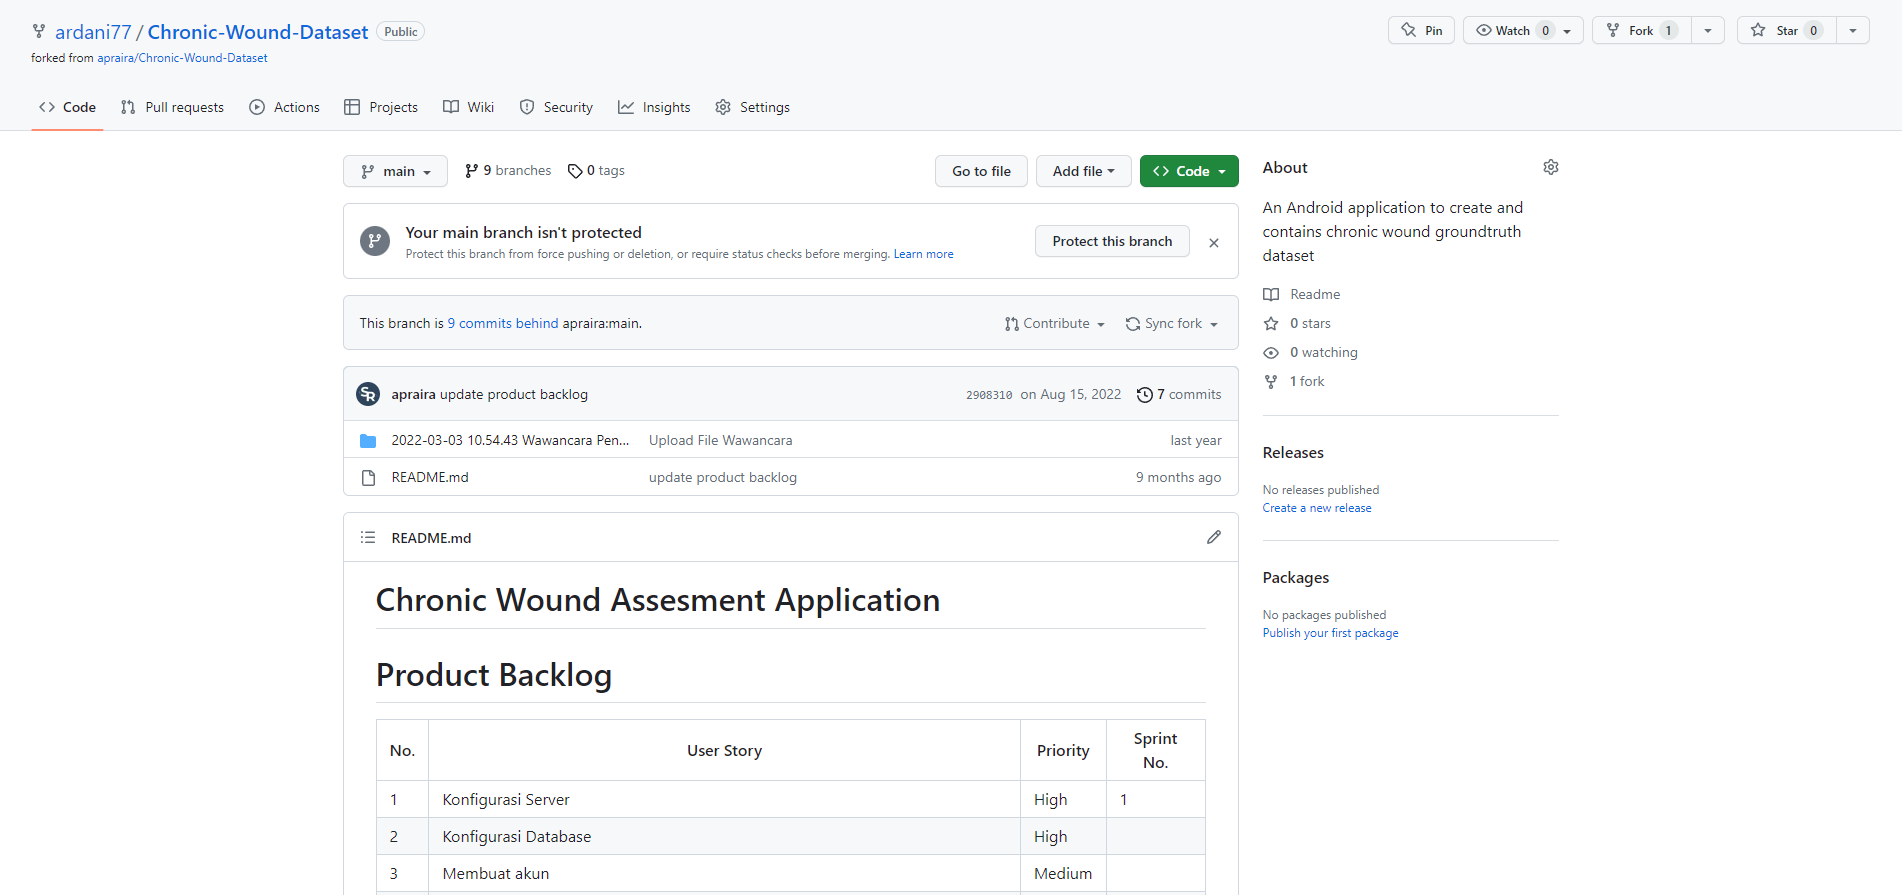
\includegraphics[keepaspectratio, width=10cm]{gambar/fork_repo}
		\caption{\textit{Fork repo frontend} dan \textit{backend} penelitian sebelumnya}
		\label{gambar:fork_repo}
	\end{figure}
	
	Setelah itu dibuatlah Mock-up UI untuk skoring lanjutan yang mana Design Styleguide mengikuti penelitian sebelumnya.
	\begin{figure}[H]
		\centering
		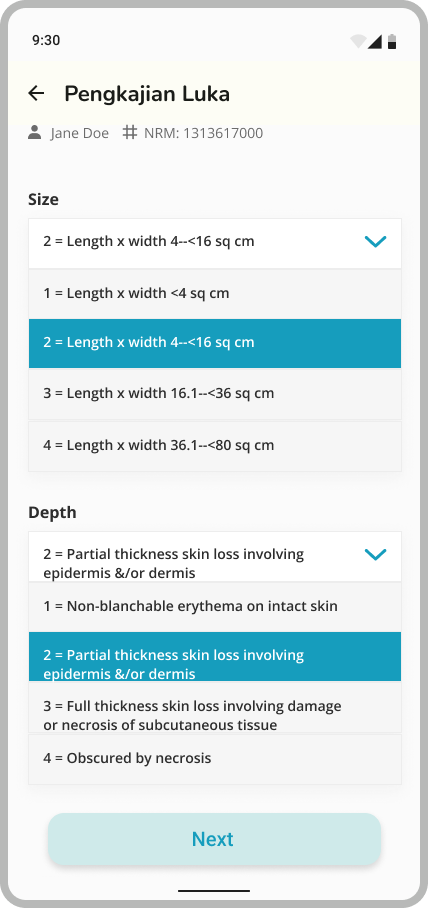
\includegraphics[keepaspectratio, width=4cm]{gambar/mockup_skoring}
		\caption{\textit{Mock-up skoring} pengkajian luka lanjutan}
		\label{gambar:mockup_skoring}
	\end{figure}
	
	\item Konversi seluruh \textit{activity} menjadi \textit{fragment}
	
	Hal selanjutnya yang dilakukan adalah mengkonversi seluruh activity yang terdapat pada penelitian sebelumnya lalu mengubahnya menjadi fragment. Diawali dengan mencatat seluruh activity yang ada pada penelitian sebelumnya.
	\begin{figure}[H]
		\centering
		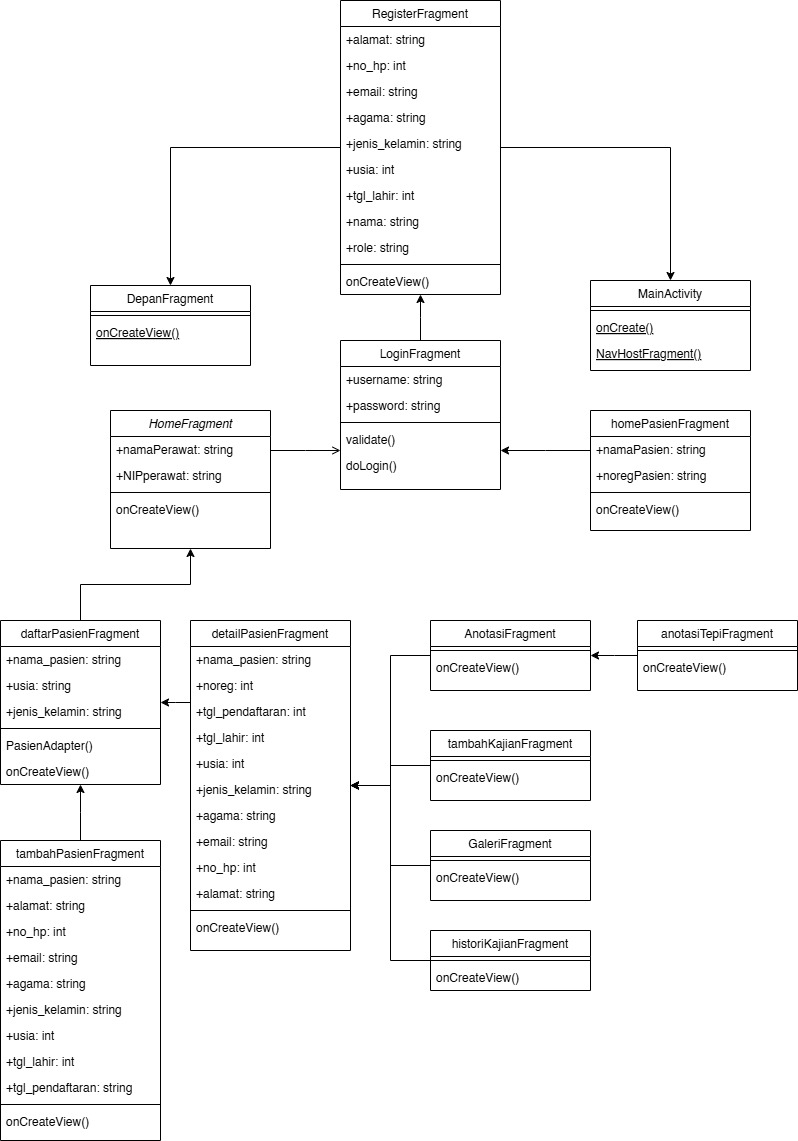
\includegraphics[keepaspectratio, width=9cm]{gambar/class_diagram}
		\caption{Class Diagram Activity}
		\label{gambar:class_diagram_activity}
	\end{figure}
	
	Setelah itu buat fragment berdasarkan catatan activity yang sudah dilakukan.
	\begin{figure}[H]
		\centering
		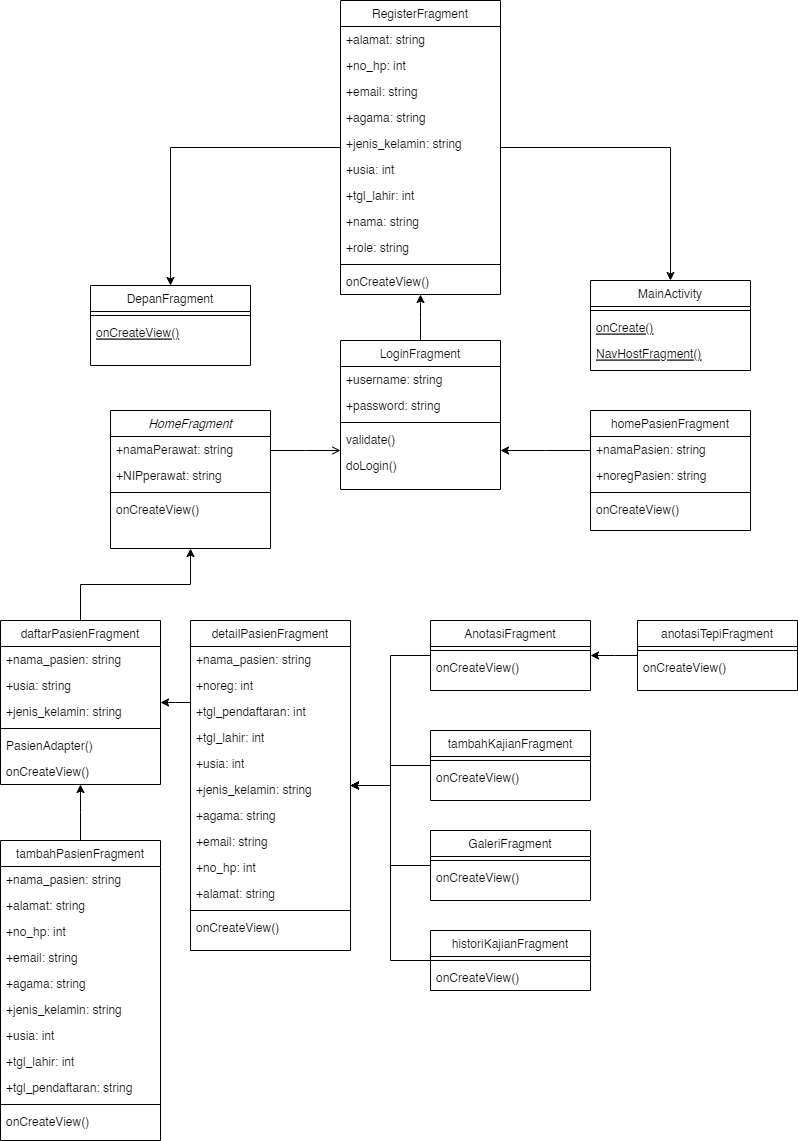
\includegraphics[keepaspectratio, width=9cm]{gambar/class_diagram_fragment}
		\caption{Class Diagram Fragment}
		\label{gambar:class_diagram_fragment}
	\end{figure}
	
	Lalu untuk menghubungkan antara satu fragment dengan fragment lainnya dibuatlah navGraph agar tersambung secara otomatis.
	\begin{figure}[H]
		\centering
		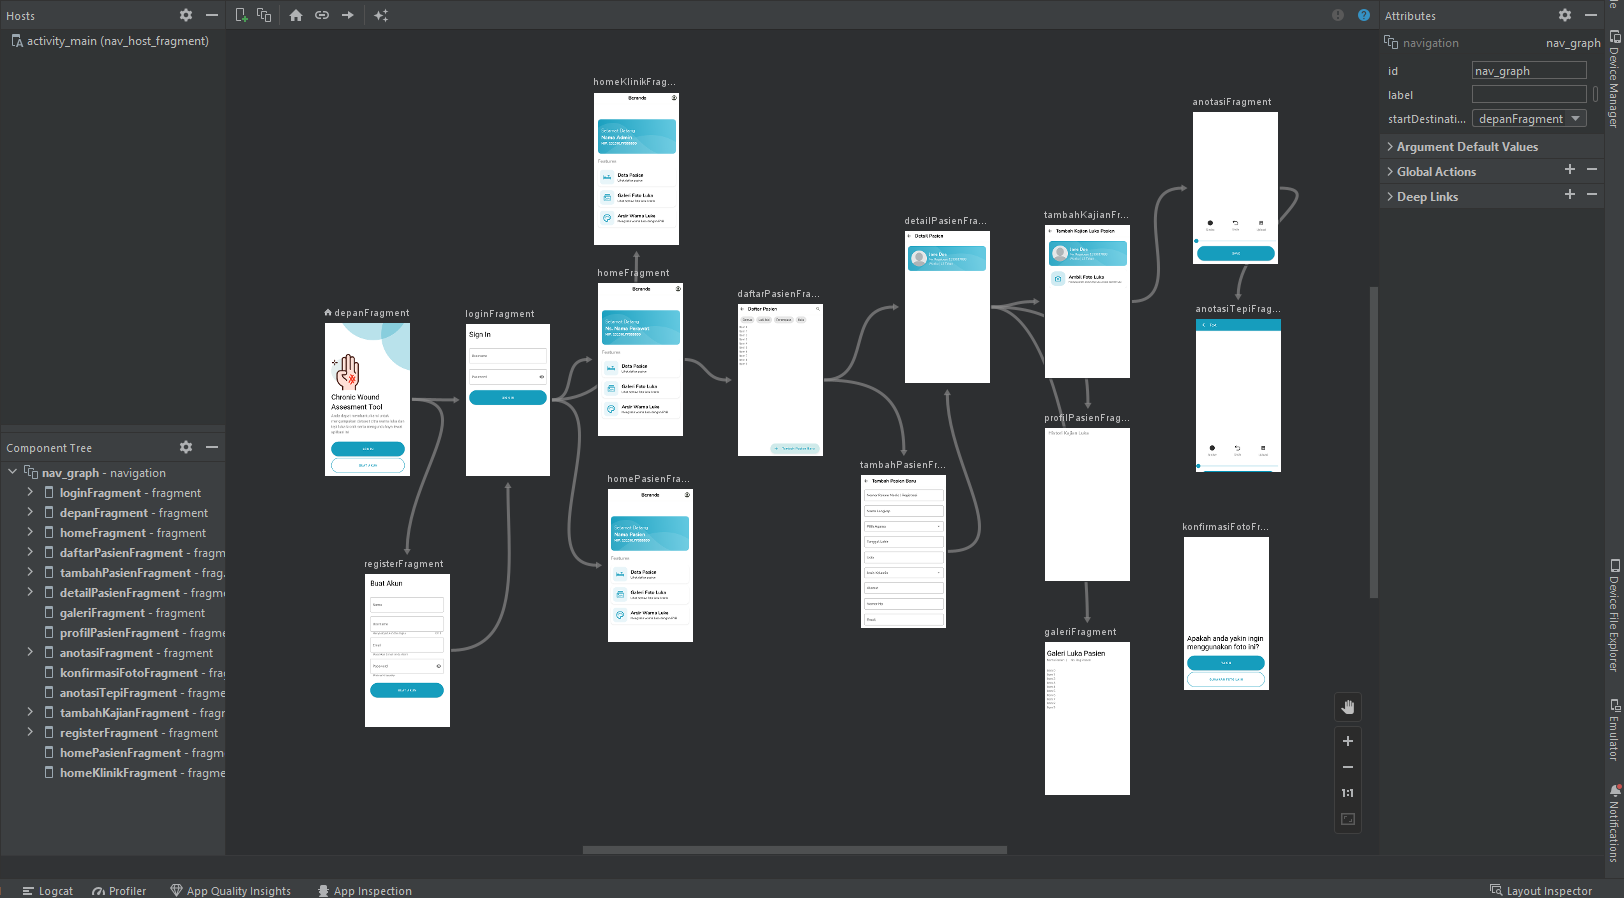
\includegraphics[keepaspectratio, width=10cm]{gambar/nav_graph}
		\caption{\textit{Navigation Graph}}
		\label{gambar:nav_graph}
	\end{figure}
	
	Selanjutnya apabila fragment telah terhubung satu sama lain dilanjutkan dengan implementasi fragment logic dari fragment login yang sudah terintegrasi dengan web service.
	
	\textit{Code fragment logic pada fragment login}
	\begin{lstlisting}
override fun onCreateView(
	inflater: LayoutInflater, container: ViewGroup?,
	savedInstanceState: Bundle?,
    ): View? {
	val root = inflater.inflate(R.layout.fragment_login, container, false)
	val formLogin = root.findViewById(R.id.formLogin) as FrameLayout
	val login = root.findViewById(R.id.buttonLogin) as Button
	val editTextUsername = root.findViewById(R.id.editTextUserName) as EditText
	val editTextPassword = root.findViewById(R.id.editTextPassword) as EditText
	val textInputLayoutUsername = root.findViewById(R.id.textInputLayoutUserName) as TextInputLayout
	val textInputLayoutPassword = root.findViewById(R.id.textInputLayoutPassword) as TextInputLayout
	formLogin.setVisibility(View.VISIBLE)

	fun validate(username: String?, password: String?): Boolean {
		if (username == null || username.trim { it <= ' ' }.length == 0) {
			textInputLayoutUsername.setError("Username tidak boleh kosong")
			return false
		}
		if (password == null || password.trim { it <= ' ' }.length == 0) {
			textInputLayoutPassword.setError("Password tidak boleh kosong")
			return false
		}
		return true
        }

	fun doLogin(username: String, password: String) {
		val retro = ApiService().getInstance().create(WoundApi::class.java)
		val coroutineExceptionHandler = CoroutineExceptionHandler{_, throwable ->
			throwable.printStackTrace()
		}
		GlobalScope.launch(Dispatchers.IO + coroutineExceptionHandler) {
			val result = retro.getLogin(username, password)
			val testRetro = result.body()
				if (result.isSuccessful)
					Log.d("data: ", result.toString())
					Log.d("body: ", result.body()!!.name)
					Log.d("test: ", testRetro.toString())
					SaveSharedPreference.setLoggedIn(requireActivity().applicationContext, true)
					val preferences: SharedPreferences = requireActivity().getSharedPreferences("preferences", Context.MODE_PRIVATE)
					val editor = preferences.edit()
					editor.putString("name", username)
					editor.commit()
					if (result.body()!!.role == "perawat") {
						findNavController().navigate(R.id.homeFragment)
					}
					else if (result.body()!!.role == "pasien") {
						findNavController().navigate(R.id.homePasienFragment)
					}
					else if (result.body()!!.role == "klinik") {
						findNavController().navigate(R.id.homeKlinikFragment)
					}
			}
		}

	login.setOnClickListener{
		val username: String = editTextUsername.text.toString()
		val password: String = editTextPassword.text.toString()
		//Check user input is correct or not
		if (validate(username, password)) {
			doLogin(username, password)
		}
	}

	return root
}
	\end{lstlisting}
	
	Pada code diatas retrofit pemanggilan juga diubah menjadi courutine. Yang diubah juga selain itu adalah database. Karena sekarang akan menerapkan sistem multiuser, dapat dipastikan bahwa database yang digunakan pun ada perubahan dibagian user. Ditambahkan kolom role pada database agar dapat memudahkan identifikasi user mana perawat dan mana yang pasien.
	\begin{figure}[H]
		\centering
		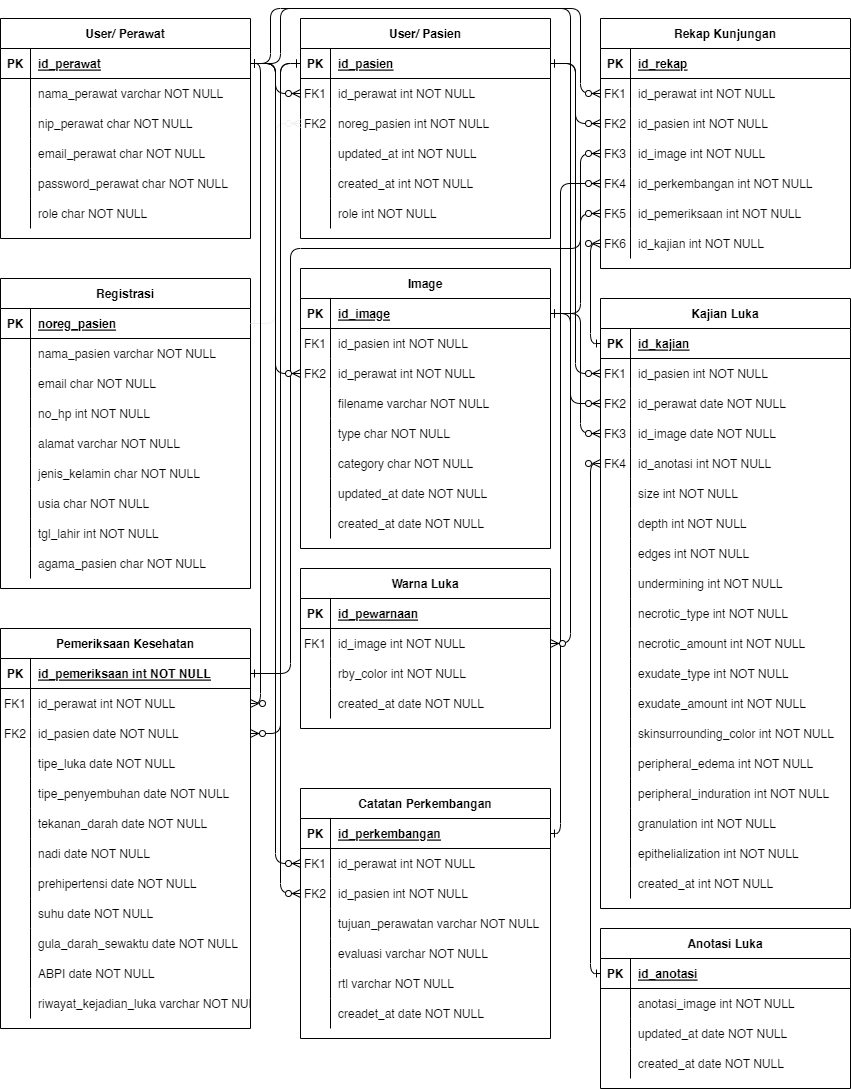
\includegraphics[keepaspectratio, width=9cm]{gambar/erd_new}
		\caption{\textit{Entity Relationship Diagram}}
		\label{gambar:erd_new}
	\end{figure}
	
	\item Login User
	
	Setelah mengubah database dengan menambahkan role, maka dilanjutkan dengan membuat dashboard user setelah login. Karena pada penelitian sebelumnya hanya terdapat dashboard perawat setelah login.
	\begin{figure}[H]
		\centering
		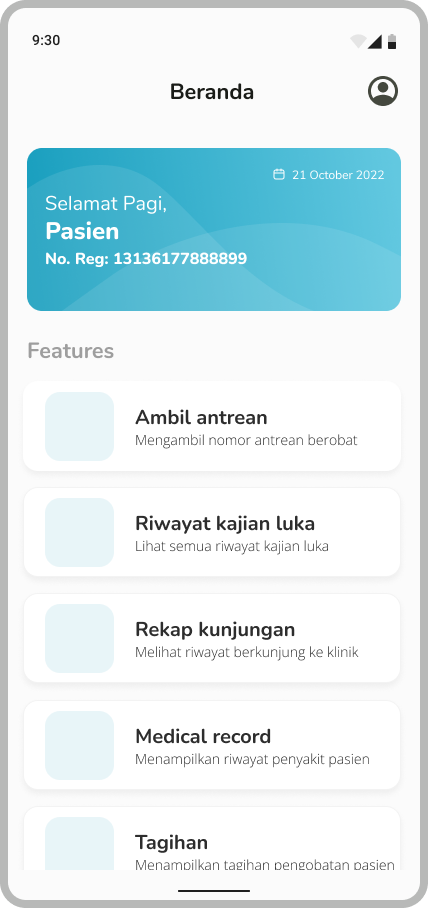
\includegraphics[keepaspectratio, width=4cm]{gambar/dashboard_user}
		\caption{\textit{Dashboard User}}
		\label{gambar:dashboard_user}
	\end{figure}
	
	\end{enumerate}
	
\subsection{\textit{Sprint 2}}
\textit{Sprint-2} pada \textit{product backlog} berisi 1 \textit{story} yaitu membuat fitur untuk evaluasi kondisi kesehatan pasien sebelum perawatan. \textit{Story} ini dipecah menjadi beberapa bagian sebagai berikut.

\begin{table}[H]
	\caption{\textit{Sprint 2}}
	\label{sprint2_backlog}
	\begin{tabular}{@{} |p{0.5cm}|p{5cm}|p{5cm}|p{2cm}| @{}}
		\hline
		\textbf{No.} & \textbf{\textit{User Story}} & \textbf{\textit{Task}} & \textbf{\textit{Status}} \\
		\hline
		\multirow{3}{3cm}{1.} & \multirow{3}{5cm}{Evaluasi kondisi kesehatan pasien sebelum perawatan} & Buat mock-up pemeriksaan kesehatan sebelum perawatan & selesai\\
		\cline{3-4}
		 & & Pengembangan backend bagian pengecekan kesehatan & selesai\\
		\cline{3-4}
		 & & Pengembangan android bagian yang mengkoneksikan dengan pengecekan kondisi pasien & selesai\\
		\cline{3-4}
		 & & Pembuatan XML Android yang mendefinisikan & selesai\\
		\hline
	\end{tabular}
	\end{table}
	
	Tujuan dari \textit{sprint-2} ini adalah untuk membuat desain halaman evaluasi kesehatan, pengembangan \textit{backend} bagian pengecekan kesehatan, lalu pembuatan dan pengembangan \textit{XML Android} terkait bagian ini. Kendala yang dialami oleh penulis ialah mengintegrasikan \textit{code} baru ini kedalam yang sudah ada.
	
\begin{enumerate}
\item \textit{Mock-up} pemeriksaan kesehatan

Hal yang pertama dilakukan ketika menjalankan \textit{sprint} ini ialah membuat desain \textit{mock-up} untuk aplikasi yang akan digunakan. \textit{Field-field} yang terdapat pada \textit{mock-up} didapatkan dari form pengkajian luka klinik moist care pada lampiran C.
	\begin{figure}[H]
		\centering
		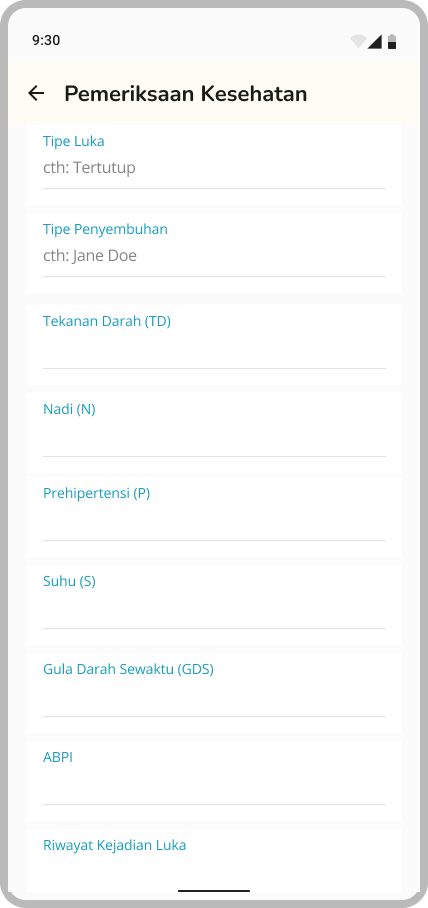
\includegraphics[keepaspectratio, width=4cm]{gambar/tampilan_pemeriksaan_kesehatan}
		\caption{\textit{Mock-up} Pemeriksaan Kesehatan}
		\label{gambar:tampilan_pemeriksaan_kesehatan}
	\end{figure}
	
	\item \textit{Class Diagram}
	
	Pada \textit{class diagram} ini menggambarkan kelas-kelas apa saja yang akan digunakan dalam sistem. Biasanya terdapat 3 kelas yaitu model, view, dan controller. Pada sprint-2 ini penulis membuat 3 kelas yaitu model yang berwarna hijau, view berwarna biru, dan controller berwarna kuning.
	\begin{figure}[H]
		\centering
		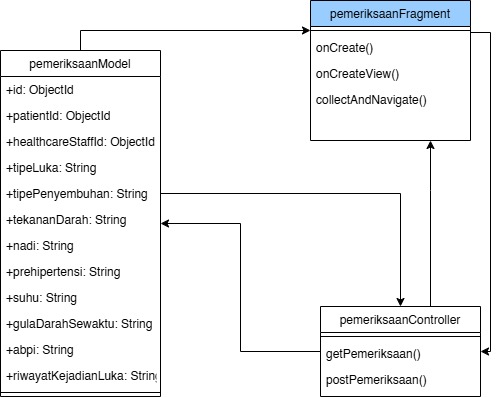
\includegraphics[keepaspectratio, width=8cm]{gambar/class_diagram_sprint_2}
		\caption{\textit{Class Diagram Sprint 2}}
		\label{gambar:class_diagram_sprint_2}
	\end{figure}
	
	
	\item \textit{Backend} bagian pengecekan kesehatan
	
	Sebelum \textit{mock-up UI} sebelumnya diterapkan, pengembangan terhadap backend terkait bagian ini dijalankan. Berikut adalah \textit{code} model dari periksaKesehatan.
	\begin{lstlisting}
def create_medical_checkup(request):
    check  = get_from_collection("patient_info",{"user_id":ObjectId(request.form["patient_id"])})
    check = json.loads(bson.json_util.dumps(list(check)))
    if len(check) == 0:
        raise Exception("Pasien tidak ditemukan")
    # data = {
    #     "patient_id" : ObjectId(request.form["patient_id"])
    # }
    check2  = get_from_collection("healthcare_staff_info",{"user_id":ObjectId(request.form["healthcare_staff_id"])})
    check2 = json.loads(bson.json_util.dumps(list(check2)))
    if len(check2) == 0:
        raise Exception("Perawat tidak ditemukan")
    data = {
        "patient_id" : ObjectId(request.form["patient_id"]),
        "healthcare_staff_id" : ObjectId(request.form["healthcare_staff_id"]), 
        "created_at" : time.strftime("%d/%m/%Y %H:%M:%S"),
        "updated_at" : time.strftime("%d/%m/%Y %H:%M:%S")
    }
    nullable = {"tipe_luka": "string",
               "tipe_penyembuhan": "string",
               "tekanan_darah": "string",
               "nadi": "string",
               "prehipertensi": "string",
               "suhu": "string",
               "gula_darah_sewaktu": "string",
               "abpi": "string",
               "riwayat_kajian_luka": "string"}
    for param in nullable.keys():
        if request.form.get(param)!='""' and request.form.get(param)!="" and request.form.get(param)!="''" and request.form.get(param)!=None:
            if nullable[param]=="string":
                data[param] = request.form[param]
            elif nullable[param]=="int":
                data[param] = int(request.form[param])
            elif nullable[param]=="date":
                data[param] = request.form[param]
            elif nullable[param]=="float":
                data[param] = float(request.form[param])
        else:
            data[param] = None
    data = insert_medical_checkup(data)
    return data.inserted_id
	\end{lstlisting}
	Dalam \textit{code} tersebut dapat diketahui bahwa pertama yang dilakukannya ialah mengecek apakah pasien dan perawat sudah terdaftar dalam server. Lalu dilanjutkan dengan mengisi field yang disediakan oleh \textit{mock-up} sebelumnya dan dimasukkan ke server. Data-data dari field yang disediakan bersifat \textit{nullable} dikarenakan pengecekan ini tidak wajib dilakukan kepada pasien yang sudah pernah berobat.
	
	\item Konfigurasi \textit{controller}
	
	Setelah dibuatnya model periksaKesehatan, dilanjutkan dengan pengembangan API Service untuk dikoneksikan dengan android.
	\textit{Controller periksaKesehatan}
	\begin{lstlisting}
@bp.route("v1/medical_checkup/",methods=["POST"])
def create_medical_checkup():
    try:
        return json.dumps({"medical_checkup_id" : str(db_pemeriksaan.create_medical_checkup(request)) })
    except Exception as ex:
        print(ex)
        return Response(response = json.dumps({"message" : f"{ex}"}), mimetype="application/json", status=500)
	\end{lstlisting}
	
	\item Pengembangan XML android dan konfigurasi
	
	Bagian terakhir dari \textit{sprint} ini ialah implementasi tampilan \textit{mock-up} yang telah dibuat ke dalam aplikasi dan diintegrasikan dengan backend yang juga telah dibuat sebelumnya.
	\begin{figure}[H]
		\centering
		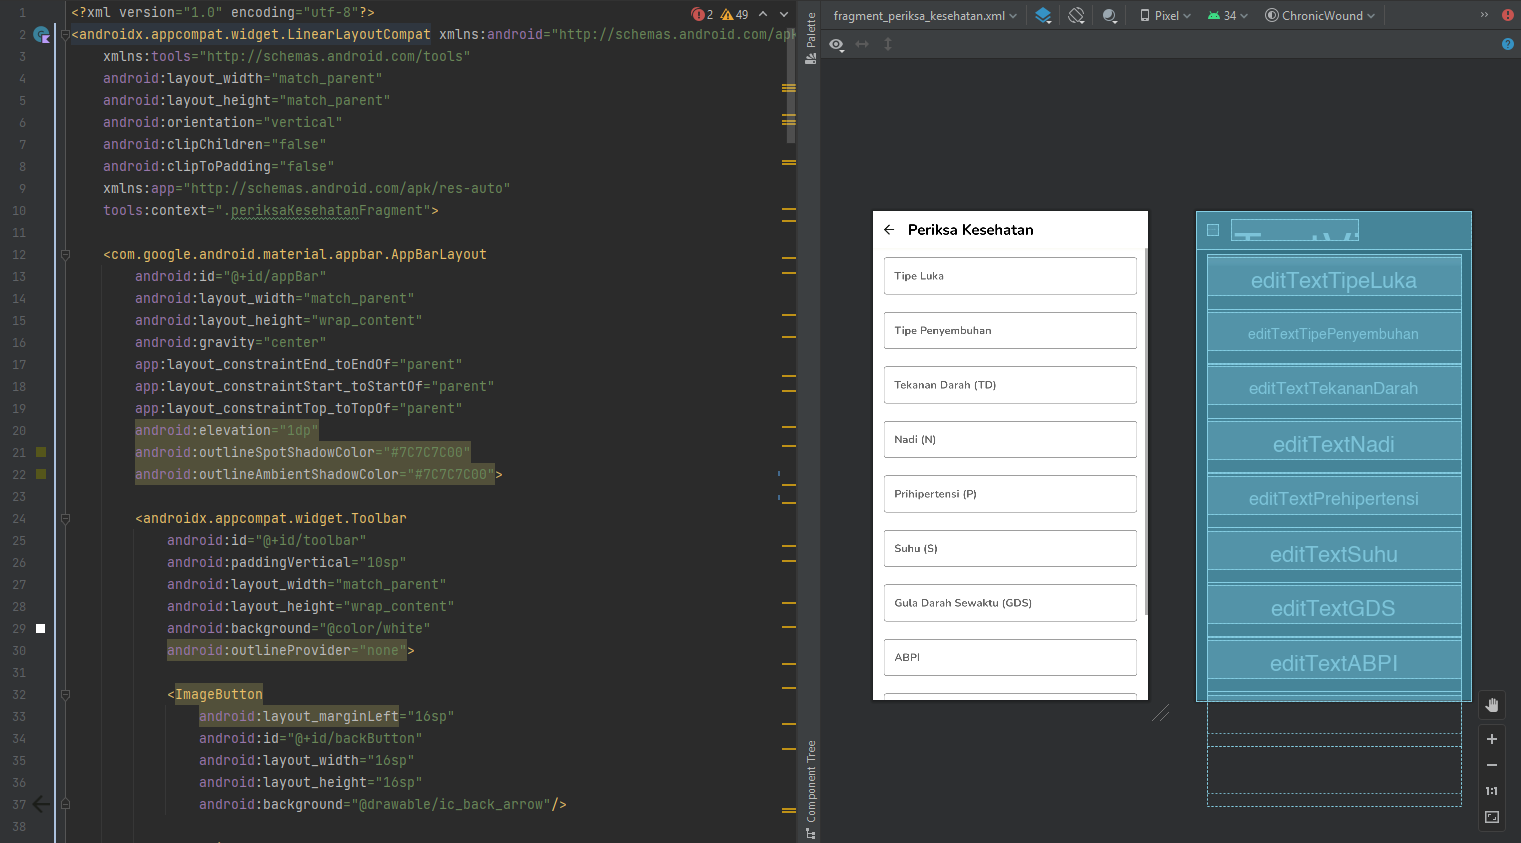
\includegraphics[keepaspectratio, width=10cm]{gambar/fragment_periksa_kesehatan}
		\caption{Fragment Pemeriksaan Kesehatan}
		\label{gambar:fragment_periksa_kesehatan}
	\end{figure}
	
	\textit{Code Konfigurasi}
	\begin{lstlisting}
override fun onCreateView(
        inflater: LayoutInflater, container: ViewGroup?,
        savedInstanceState: Bundle?,
    ): View? {
        // Inflate the layout for this fragment
        val root = inflater.inflate(R.layout.fragment_periksa_kesehatan, container, false)
        val nextButton = root.findViewById(R.id.buttonSubmit) as Button
        val tipeLuka = root.findViewById(R.id.editTextTipeLuka) as EditText
        val tipePenyembuhan = root.findViewById(R.id.editTextTipePenyembuhan) as EditText
        val tekananDarah = root.findViewById(R.id.editTextTekananDarah) as EditText
        val nadi = root.findViewById(R.id.editTextNadi) as EditText
        val prehipertensi = root.findViewById(R.id.editTextPrehipertensi) as EditText
        val suhu = root.findViewById(R.id.editTextSuhu) as EditText
        val gulaDarahSewaktu = root.findViewById(R.id.editTextGDS) as EditText
        val abpi = root.findViewById(R.id.editTextABPI) as EditText
        val riwayatKejadianLuka = root.findViewById(R.id.editTextRiwayatKejadian) as EditText
        val backButton = root.findViewById(R.id.backButton) as ImageButton
        val patient_id = arguments?.getString("patient_id")
        val healthcare_staff_id = arguments?.getString("healthcare_staff_id")
        val namaPasien = arguments?.getString("namaPasien")
        val nomorRekamMedis = arguments?.getString("nomorRekamMedis")
        val usiaPasien = arguments?.getString("usiaPasien")
        val jenisKelamin = arguments?.getString("jenisKelamin")
        tipeLuka.setText(arguments?.getString("tipe_luka") ?: "")
        tipePenyembuhan.setText(arguments?.getString("tipe_penyembuhan") ?: "")
        tekananDarah.setText(arguments?.getString("tekanan_darah") ?: "")
        nadi.setText(arguments?.getString("tekanan_nadi") ?: "")
        prehipertensi.setText(arguments?.getString("tekanan_prehipertensi") ?: "")
        suhu.setText(arguments?.getString("suhu_tubuh") ?: "")
        gulaDarahSewaktu.setText(arguments?.getString("gula_darah_sewaktu") ?: "")
        abpi.setText(arguments?.getString("abp_i") ?: "")
        riwayatKejadianLuka.setText(arguments?.getString("riwayat_kejadian_luka") ?: "")
        nextButton.setOnClickListener{
            val tipe_luka: String = tipeLuka.text.toString()
            val tipe_penyembuhan: String = tipePenyembuhan.text.toString()
            val tekanan_darah: String = tekananDarah.text.toString()
            val tekanan_nadi: String = nadi.text.toString()
            val tekanan_prehipertensi: String = prehipertensi.text.toString()
            val suhu_tubuh: String = suhu.text.toString()
            val gula_darah_sewaktu: String = gulaDarahSewaktu.text.toString()
            val abp_i: String = abpi.text.toString()
            val riwayat_kejadian_luka: String = riwayatKejadianLuka.text.toString()
            println("tipe_luka:$tipe_luka")
            //Check user input is correct or not
            if (validate(tipe_luka, tipe_penyembuhan, tekanan_darah, tekanan_nadi, tekanan_prehipertensi, suhu_tubuh, gula_darah_sewaktu, abp_i, riwayat_kejadian_luka)) {
                //do periksa kesehatan
                val action = periksaKesehatanFragmentDirections.actionPeriksaKesehatanFragmentToTambahKajianFragment()
                findNavController().navigate(action)
            }
        }
        return root
    }
	\end{lstlisting}
	

\end{enumerate}

\subsection{\textit{Sprint 3}}
\textit{Sprint-3} kali ini sama seperti \textit{sprint} sebelumnya yaitu berisi 1 \textit{story} terkait fitur rekap kunjungan pasien. \textit{Story} ini memiliki beberapa \textit{task} sebagai berikut.
\begin{table}[H]
	\caption{\textit{Sprint 3}}
	\label{sprint3_backlog}
	\begin{tabular}{@{} |p{0.5cm}|p{5cm}|p{5cm}|p{2cm}| @{}}
		\hline
		\textbf{No.} & \textbf{\textit{User Story}} & \textbf{\textit{Task}} & \textbf{\textit{Status}} \\
		\hline
		\multirow{3}{3cm}{1.} & \multirow{3}{5cm}{Rekap kunjungan pasien} & Identifikasi kebutuhan pengguna terkait fitur rekap kunjungan pasien & selesai\\
		\cline{3-4}
		 & & Mendesain struktur database untuk menyimpan data kunjungan pasien & selesai\\
		\cline{3-4}
		 & & Mendesain tampilan rekap kunjungan pasien & selesai\\
		\cline{3-4}
		 & & Mengembangkan tampilan daftar kunjungan pasien di aplikasi & selesai\\
		 \cline{3-4}
		 & & Menghubungkan tampilan dengan API untuk mengambil data kunjungan & selesai\\
		\hline
	\end{tabular}
	\end{table}
Pada \textit{sprint} ini \textit{story} yang dipilih untuk diuraikan adalah membuat fitur rekap kunjungan pasien. Tujuan dari \textit{sprint} ini ialah untuk membuat fitur rekap kunjungan pasien, pengembangan struktur database, desain tampilan dan implementasi kedalam aplikasi. Kendala yang dialami oleh penulis pada \textit{sprint} ini adalah mengembakan struktur database yang ada saat ini.

\begin{enumerate}
\item Analisis data yang diperlukan untuk menampilkan rekap kunjungan

Identifikasi kebutuhan pengguna terkait fitur rekap kunjungan pasien. Diskusi dengan \textit{scrum master} mengenai format dan informasi yang ditampilkan dalam rekap kunjungan. Serta analisis data yang diperlukan berdasarkan pada lampiran C.
\item Struktur database untuk menyimpan data kunjungan pasien

Selanjutnya yaitu mengembangkan database pada fitur rekap kunjungan pasien. Masukkan data rekap kunjungan pasien pada erd yang sudah dirancang.
	\begin{figure}[H]
		\centering
		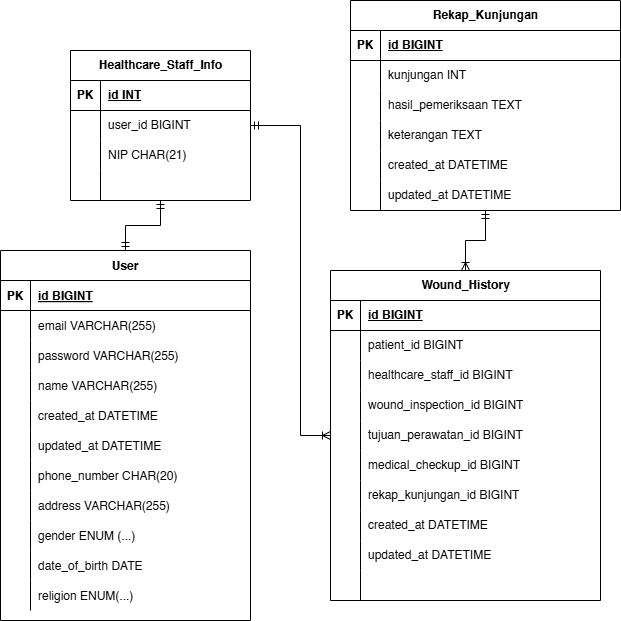
\includegraphics[keepaspectratio, width=8cm]{gambar/erd_sprint_3}
		\caption{\textit{ERD Sprint-3}}
		\label{gambar:erd_sprint_3}
	\end{figure}
\item Desain tampilan rekap kunjungan pasien

Setelah database dirancang dilanjutkan dengan membuat tampilan daftar kunjungan pasien di aplikasi. Isi dari konten berdasarkan diskusi dengan \textit{scrum master} dan data pada lampiran C.
	\begin{figure}[H]
		\centering
		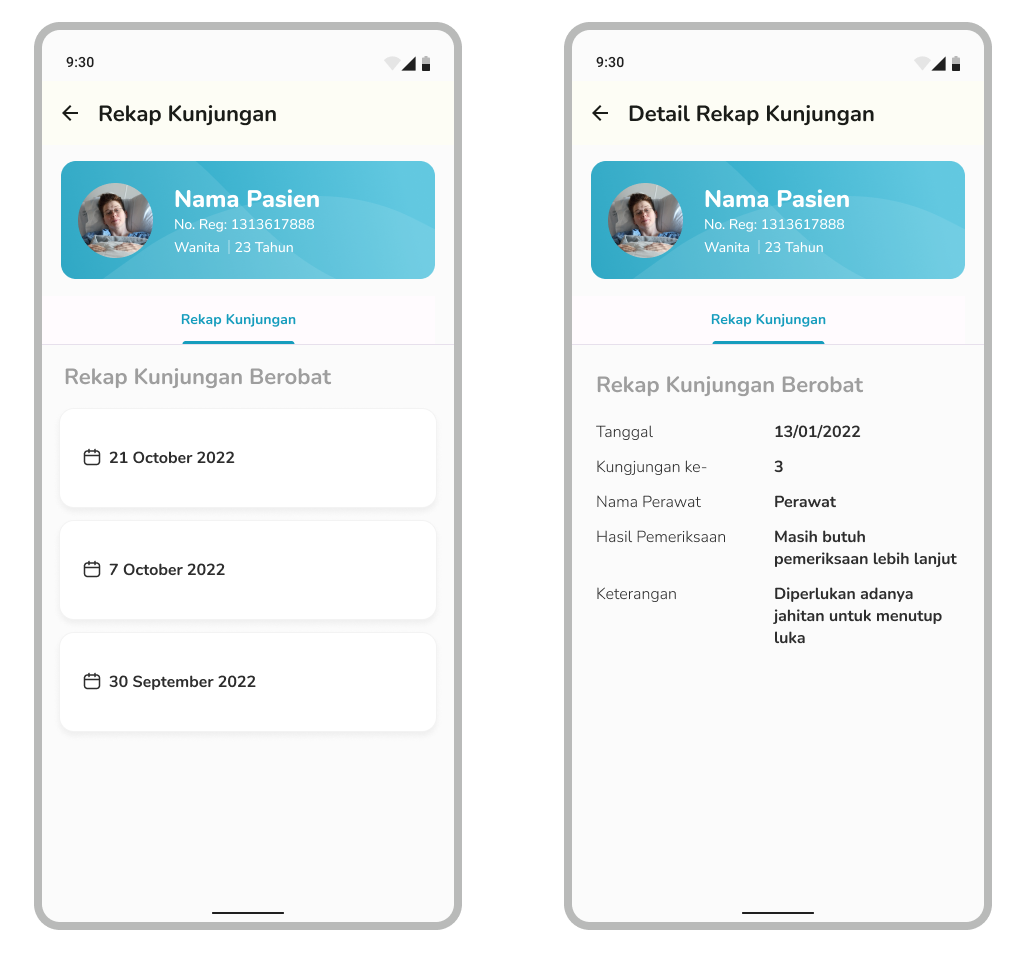
\includegraphics[keepaspectratio, width=8cm]{gambar/tampilan_rekap_kunjungan}
		\caption{\textit{Mock-up} Rekap Kunjungan}
		\label{gambar:tampilan_rekap_kunjungan}
	\end{figure}

\item Pengembangan tampilan daftar kunjungan pasien pada aplikasi dan konfigurasi

\textit{Sprint} ini diakhiri dengan mengembangkan tampilan daftar kunjungan pasien pada aplikasi dan konfigurasinya. Tampilan rekap kunjungan pasien berdasarkan \textit{mock-up} sebelumnya dan konfigurasi berdasarkan rancangan database yang telah dibuat.
\textit{Code konfigurasi rekap kunjungan}
\begin{lstlisting}
class pasienRekapKunjunganFragment : Fragment() {
    private var _binding: FragmentPasienRekapKunjunganBinding? = null
    private val binding get() = _binding!!
    private lateinit var patient_id: String
    private lateinit var recyclerView: RecyclerView
    private lateinit var adapter: pasienRekapKunjunganAdapter
    private var kunjunganArrayList: ArrayList<PasienRekapKunjunganItem> = ArrayList()

    override fun onViewCreated(view: View, savedInstanceState: Bundle?) {
        super.onViewCreated(view, savedInstanceState)

        patient_id = arguments?.getString("patient_id")!!
        val namaPasien = arguments?.getString("nama")
        val NRMpasien = arguments?.getString("nrm")
        binding.backButton.setOnClickListener {
            val action = pasienRekapKunjunganFragmentDirections.actionPasienRekapKunjunganFragmentToHomePasienFragment()
            action.arguments.putString("patient_id", patient_id)
            action.arguments.putString("nama", namaPasien)
            action.arguments.putString("nrm", NRMpasien)
            findNavController().navigate(action)
        }
        cariPasien(patient_id)
        getPasienRekapKunjungan(patient_id)
        recyclerView = binding.recyclerView
        recyclerView.layoutManager = LinearLayoutManager(context)
        adapter = pasienRekapKunjunganAdapter(kunjunganArrayList, patient_id, namaPasien ?: "", NRMpasien ?: "")
        recyclerView.adapter = adapter
    }
}
\end{lstlisting}
\end{enumerate}

\subsection{\textit{Sprint 4}}
Pada \textit{sprint-4} ini terdapat 1 \textit{story} yaitu untuk mencatat perkembangan pasien dan diagnosis agar dapat menentukan langkah penyembuhan selanjutnya secara lebih efektif. \textit{Sprint} ini diuraikan menjadi beberapa bagian sebagai berikut.
	\begin{table}[H]
	\caption{\textit{Sprint 4}}
	\label{sprint4_backlog}
	\begin{tabular}{@{} |p{0.5cm}|p{5cm}|p{5cm}|p{2cm}| @{}}
		\hline
		\textbf{No.} & \textbf{\textit{User Story}} & \textbf{\textit{Task}} & \textbf{\textit{Status}} \\
		\hline
		\multirow{3}{3cm}{1.} & \multirow{3}{5cm}{Catatan perkembangan/ diagnosis untuk langkah penyembuhan selanjutnya} & \textit{Requirement Gathering dan Analysis} & selesai\\
		\cline{3-4}
		 & & \textit{Database dan API Development} & selesai\\
		\cline{3-4}
		 & & \textit{UI Design} & selesai\\
		\cline{3-4}
		 & & \textit{Frontend Development} & selesai\\
		\hline
	\end{tabular}
	\end{table}
Tujuan \textit{Sprint-4} ini adalah membuat fitur catatan perkembangan dan diagnosis untuk langkah penhembuhan selanjutnya. Pada \textit{sprint} ini identifikasi kebutuhan, mendesain struktur database dan implementasi, mendesain tampilan input catatan perkembangan dan diagnosis pasien, serta menghubungkan tampilan dengan API untuk menyimpan dan menampilkan data catatan perkembangan.

\begin{enumerate}
\item \textit{Requirement Gathering dan Analysis}

Identifikasi kebutuhan pengguna terkait fitur "Tujuan Perawatan". Diskusi dengan \textit{scrum master} mengenai informasi yang perlu dicatat (diagnosis, perkembangan, tindakan lanjutan). Analisis data yang diperlukan untuk mendukung fitur ini berdasar dari formulir pada lampiran C menjadi pijakan untuk langkah selanjutnya.

\item \textit{Database dan API Development}

Pada \textit{task} ini penulis mendesain struktur database untuk menyimpan catatan perkembangan dan diagnosis. Mengembangkan endpoint API untuk mencatat dan mengambil data tujuan perawatan. dan diakhiri implementasi validasi input untuk memastikan data yang dimasukkan akurat.
	\begin{figure}[H]
		\centering
		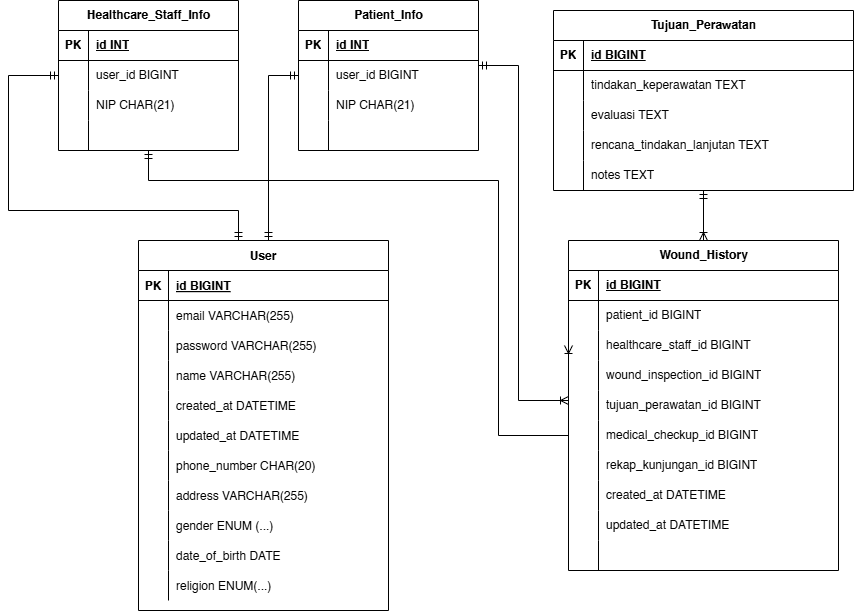
\includegraphics[keepaspectratio, width=9cm]{gambar/erd_sprint_4}
		\caption{\textit{ERD Sprint-4}}
		\label{gambar:erd_sprint_4}
	\end{figure}
\textit{Endpoint API}
\begin{lstlisting}
@bp.route("v1/tujuan_perawatan/", methods=["POST"])
def create_tujuan_perawatan():
    try:
        return json.dumps({"tujuan_perawatan_id" : str(db_tujuan_perawatan.create_tujuan_perawatan(request)) })
    except Exception as ex:
        print(ex)
        return Response(response = json.dumps({"message" : f"{ex}"}), mimetype="application/json", status=500)
    
@bp.route("v1/tujuan_perawatan/<id_tujuan_perawatan>", methods=["GET"])
def get_tujuan_perawatan_by_id(id_tujuan_perawatan):
    try:
        return db_tujuan_perawatan.get_tujuan_perawatan_by_id(id_tujuan_perawatan)
    except Exception as ex:
        print(ex)
        return Response(response = json.dumps({"message" : f"{ex}"}), mimetype="application/json", status=500)
\end{lstlisting}
\textit{Implementasi validasi input}
\begin{lstlisting}
def create_tujuan_perawatan(request):
    check  = get_from_collection("patient_info",{"user_id":ObjectId(request.form["patient_id"])})
    check = json.loads(bson.json_util.dumps(list(check)))
    if len(check) == 0:
        raise Exception("Pasien tidak ditemukan")
    check2  = get_from_collection("healthcare_staff_info",{"user_id":ObjectId(request.form["healthcare_staff_id"])})
    check2 = json.loads(bson.json_util.dumps(list(check2)))
    if len(check2) == 0:
        raise Exception("Perawat tidak ditemukan")
    data = {
        "patient_id" : ObjectId(request.form["patient_id"]),
        "healthcare_staff_id" : ObjectId(request.form["healthcare_staff_id"]),
        "created_at" : time.strftime("%d/%m/%Y %H:%M:%S"),
        "updated_at" : time.strftime("%d/%m/%Y %H:%M:%S")
    }
    nullable = {"tindakan_keperawatan": "list",
               "evaluasi": "string",
               "rencana_tindakan_lanjutan": "string",
               "notes": "string"}
    for param in nullable.keys():
        if request.form.get(param)!='""' and request.form.get(param)!="" and request.form.get(param)!="''" and request.form.get(param)!=None:
            if nullable[param]=="string":
                data[param] = request.form[param]
            elif nullable[param]=="int":
                data[param] = int(request.form[param])
            elif nullable[param]=="float":
                data[param] = request.form[param]
            elif nullable[param] == "list":
                try:
                    # Parsing JSON ke list
                    data[param] = json.loads(request.form[param])  # Parsing JSON ke list
                    # Verifikasi bahwa data adalah list dan semua elemen dalam list adalah string
                    if not isinstance(data[param], list):
                        raise Exception(f"Format {param} harus berupa array (list) JSON")
                    for item in data[param]:
                        if not isinstance(item, str):
                            raise Exception(f"Semua elemen dalam {param} harus berupa string")
                except json.JSONDecodeError:
                    raise Exception(f"Format {param} harus berupa array JSON yang valid")
        else:
            data[param] = None
    data = insert_tujuan_perawatan(data)
    return data.inserted_id
\end{lstlisting}

\item \textit{UI Design}

Mendesain tampilan input catatan perkembangan dan diagnosis pasien. Menentukan elemen UI seperti formulir input, daftar catatan sebelumnya, dan tombol navigasi. Serta review desain dengan \textit{scrum master}.
	\begin{figure}[H]
		\centering
		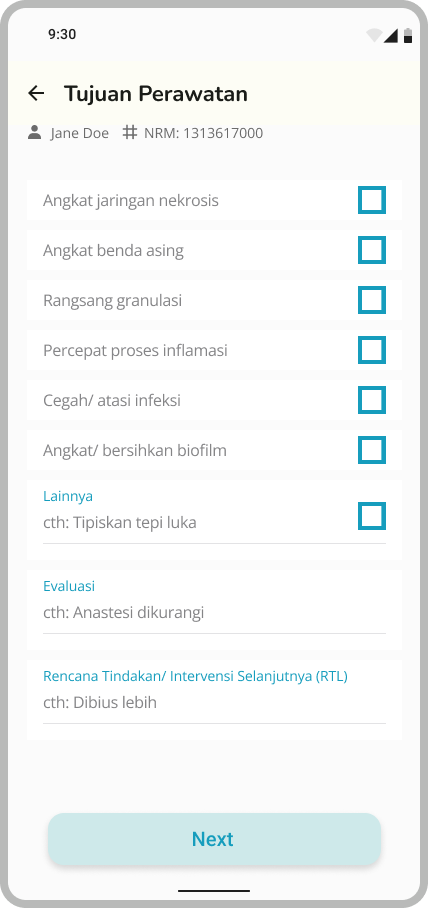
\includegraphics[keepaspectratio, width=3cm]{gambar/tampilan_tujuan_perawatan}
		\caption{\textit{UI Design} Tujuan Perawatan}
		\label{gambar:tampilan_tujuan_perawatan}
	\end{figure}
\item \textit{Frontend Development}

Mengembangkan tampilan formulir untuk memasukkan catatan perkembangan. Menampilkan daftar catatan sebelumnya agar tenaga medis dapat melihat riwayat perawatan pasien. Menghubungkan tampilan dengan API untuk menyimpan dan menampilkan data catatan perkembangan.
	\begin{figure}[H]
		\centering
		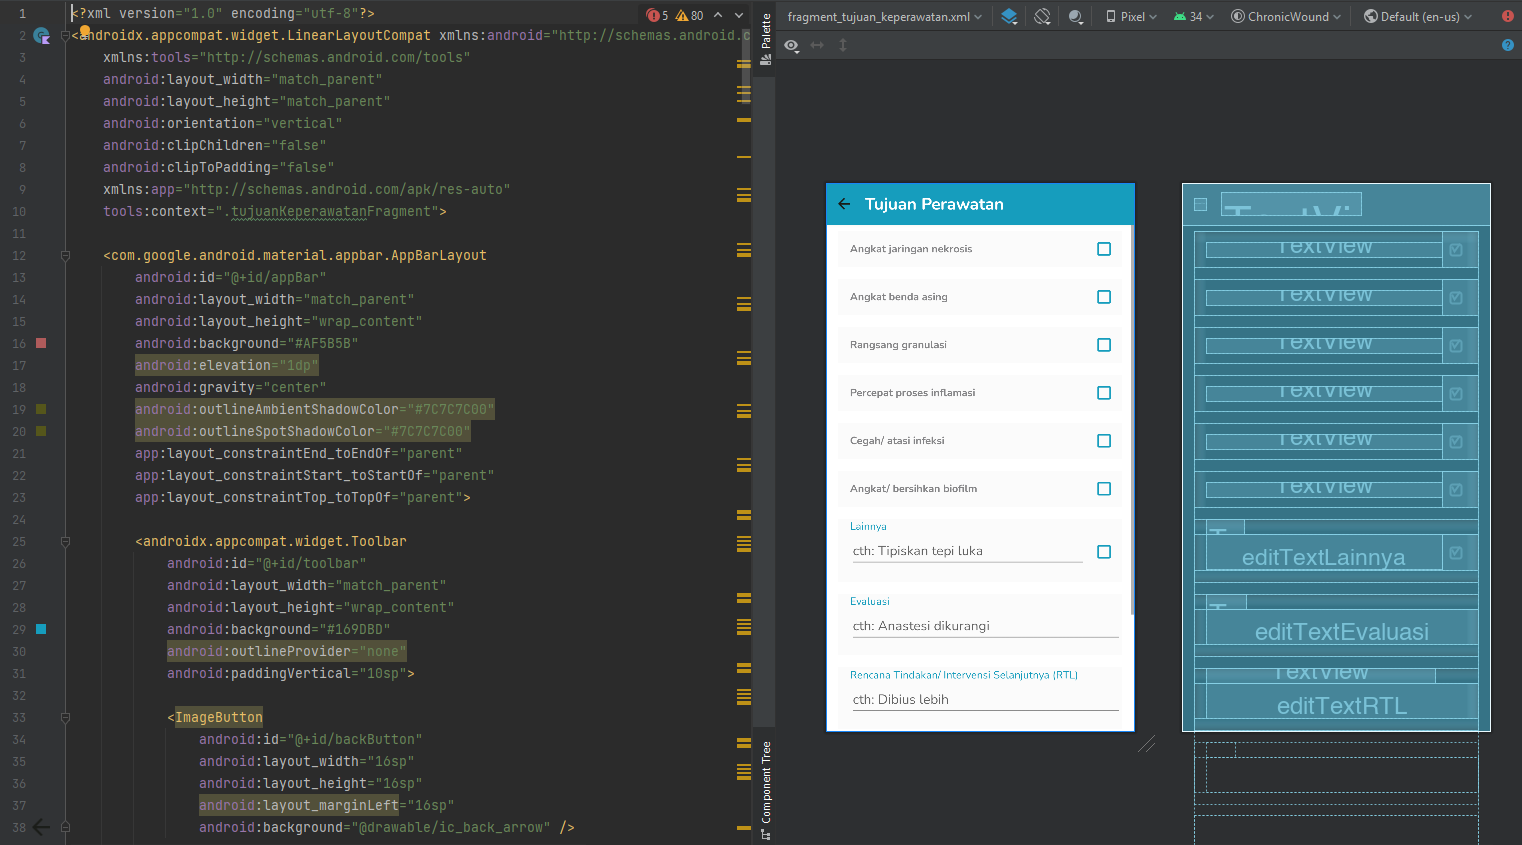
\includegraphics[keepaspectratio, width=10cm]{gambar/fragment_tujuan_perawatan}
		\caption{Fragment Tujuan Perawatan}
		\label{gambar:fragment_tujuan_perawatan}
	\end{figure}

\end{enumerate}

\subsection{\textit{Sprint 5}}
Pada \textit{Sprint} kali ini terdapat 3 \textit{story} yang berisi implementasi web service program warna luka, implementasi web service anotasi luka, dan mengembangkan progres penyembuhan luka pasien penelitian sebelumnya.
	\begin{table}[H]
	\caption{\textit{Sprint 5}}
	\label{sprint5_backlog}
	\begin{tabular}{@{} |p{0.5cm}|p{5cm}|p{5cm}|p{2cm}| @{}}
		\hline
		\textbf{No.} & \textbf{\textit{User Story}} & \textbf{\textit{Task}} & \textbf{\textit{Status}} \\
		\hline
		\multirow{3}{3cm}{1.} & \multirow{3}{5cm}{Implementasi web service program warna luka} & Meninjau kembali hasil penelitian sebelumnya mengenai web service warna luka & tidak selesai\\
		\cline{3-4}
		 & & Menganalisis kebutuhan data warna luka yang akan digunakan dalam sistem & tidak selesai\\
		\hline
		\multirow{3}{3cm}{2.} & \multirow{3}{5cm}{Implementasi web service program warna luka} & Kajian Sistem dan Identifikasi Kebutuhan & selesai\\
		\cline{3-4}
		 & & Menghubungkan API anotasi luka dengan sistem utama & selesai\\
		\cline{3-4}
		& & Menyesuaikan struktur database untuk menampung informasi anotasi yang lebih kompleks & selesai\\
		\cline{3-4}
		& & Konfigurasi tampilan anotasi penelitian sebelumnya & selesai\\
		\cline{3-4}
		& & Menampilkan riwayat anotasi berupa tampilan aplikasi & selesai\\
		\hline
		\multirow{3}{3cm}{3.} & \multirow{3}{5cm}{Mengembangkan progres penyembuhan luka pasien penelitian sebelumnya} & Menentukan parameter utama yang mencerminkan perkembangan penyembuhan luka & selesai\\
		\cline{3-4}
		 & & Merancang skema database yang dapat menyimpan riwayat progres luka pasien & selesai\\
		\cline{3-4}
		& & Mengembangkan API untuk input dan pengambilan data progres penyembuhan luka & selesai\\
		\hline
	\end{tabular}
	\end{table}
	
Tujuan dari \textit{sprint} kali ini ialah agar dapat mengidentifikasi kondisi luka dengan lebih akurat, dapat menandai area spesifik pada luka untuk dokumentasi dan analisis lebih lanjut, dan melihat perkembangan penyembuhan luka pasien secara berkala agar perawat dapat menilai efektivitas perawatan yang diberikan. Kendala yang dialami penulis pada \textit{sprint} ini ialah belum dapat menampilkan riwayat anotasi pada aplikasi dalam bentuk gambar.
\begin{enumerate}


\item Meninjau kembali hasil penelitian sebelumnya mengenai web service warna luka

Setelah ditinjau kembali hasil penelitian sebelumnya, masih terdapat banyak kekurangan yang membuat tidak memungkinkan mengintegrasi penelitian tersebut kedalam aplikasi. Oleh karena itu \textit{story} mengenai implementasi web service program warna luka ditunda hingga menemukan penelitian yang memungkinkan.
\item Kajian Sistem dan Identifikasi Kebutuhan

Meneliti mekanisme anotasi luka dalam penelitian sebelumnya. Kebutuhan sistem untuk menyimpan dan memproses anotasi luka ialah untuk. Memahami format data anotasi yang digunakan dalam penelitian sebelumnya yaitu berupa koordinat dari gambar. Menyesuaikan format penyimpanan anotasi agar kompatibel dengan sistem yang dikembangkan.
\item Menghubungkan API anotasi luka dengan sistem utama

Memastikan bahwa data anotasi dapat disimpan dan diambil kembali tanpa kendala. Menyesuaikan struktur database untuk menampung informasi anotasi yang lebih kompleks.
\textit{Implementasi}
\begin{lstlisting}
def create_annotation(path,request):
    data = {}
    nullable = {"manual_annotation": "vector_list", "minor_axis": "vector_list", "major_axis": "vector_list","circle_center":"vector","radius": "float"}
    for param in nullable.keys():
        if request.form.get(param)!='""' and request.form.get(param)!="" and request.form.get(param)!="''" and request.form.get(param)!=None:
            print(param,request.form.get(param))
            if nullable[param]== "float":
                data[param] = float(request.form[param])
            elif nullable[param] == "vector_list" or nullable[param] == "vector":
                data[param] = ast.literal_eval(request.form[param])
    check = ["circle_center","radius"]
    gate=True
    for param in check:
        if request.form.get(param)!='""' and request.form.get(param)!="" and request.form.get(param)!="''" and request.form.get(param)!=None:
            continue
        gate=False
    if gate:
        data["automatic_annotation"] = utils.automatic_annotation(path,data["circle_center"][0],data["circle_center"][1],data["radius"])
    return insert_to_collection("wound_annotation",data)
    
def automatic_annotation(path, cc, cr, rad):
    my_dpi = 96
    img = imread(path)
    im_gray = rgb2gray(img)
    im_gt = imread(path)
    sigma=3.5
    sample=400
    alpha = 0.015
    beta = 10
    gamma = 0.001 # time step
    max_num_iter=500
    theta = np.linspace(0, 2*np.pi, sample)
    r = cr + rad*np.sin(theta)
    c = cc + rad*np.cos(theta)
    snake_init = np.array([r, c]).T
    snake_xy = snake_init[:, ::-1]
    x = snake_xy[:, 0].astype(float)
    y = snake_xy[:, 1].astype(float)
    n = len(x)
    ext = gaussian(im_gray, sigma)
    ext = img_as_float(ext)
    ext = ext.astype(float, copy=False)
    ext = sobel(ext)
    a = beta
    b = -(4*beta + alpha)
    c = 6*beta + 2*alpha
    eye_n = np.eye(n, dtype=float)
    c_axis = c * eye_n
    b_axis = b * ( np.roll(eye_n, -1, axis=0) + np.roll(eye_n, -1, axis=1) )
    a_axis = a * ( np.roll(eye_n, -2, axis=0) + np.roll(eye_n, -2, axis=1) )
    A = c_axis + b_axis + a_axis
    inv = np.linalg.inv(A + gamma * eye_n)
    inv = inv.astype(float, copy=False)
    gy, gx = np.gradient(ext)
    intp1 = RectBivariateSpline(np.arange(gx.shape[1]),
                                np.arange(gx.shape[0]),
                                gx.T, kx=2, ky=2, s=0)
    intp2 = RectBivariateSpline(np.arange(gy.shape[1]),
                                np.arange(gy.shape[0]),
                                gy.T, kx=2, ky=2, s=0)
    max_px_move=1.0
    xt = np.copy(x)
    yt = np.copy(y)
    for i in range(max_num_iter):
            fx = intp1(xt, yt, dx=0, grid=False).astype(float, copy=False)
            fy = intp2(xt, yt, dy=0, grid=False).astype(float, copy=False)
            xn = np.dot(inv, gamma * xt + fx)
            yn = np.dot(inv, gamma * yt + fy)
            dx = max_px_move * np.tanh(xn - xt)
            dy = max_px_move * np.tanh(yn - yt)
            xt += dx
            yt += dy
    snake_final = np.array([xt, yt]).T
    return snake_final.tolist()
\end{lstlisting}

\item Konfigurasi tampilan anotasi penelitian sebelumnya
	
Pada penelitian Salsa sebelumnya terdapat program anotasi manual yang hasilnya menyimpan gambar anotasi manual tersebut pada aplikasi. Lalu penulis mengkonfigurasi program tersebut menjadi menyimpan titik koordinatnya dan integrasi dengan webservice anotasi luka yang sedang dibuat.
	\begin{figure}[H]
		\centering
		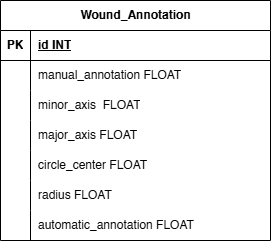
\includegraphics[keepaspectratio, width=3cm]{gambar/database_sprint_5}
		\caption{Database \textit{Sprint-5}}
		\label{gambar:database_sprint_5}
	\end{figure}
\item Menampilkan riwayat anotasi berupa tampilan aplikasi

Penulis mengalami kendala dalam menjalankan \textit{task} ini dikarenakan waktu yang kurang cukup. Selain itu, akurasi dari program yang dibuat belum akurat. Maka dari itu pada bagian ini butuh pengembangan lebih lanjut.
\item Menentukan parameter utama yang mencerminkan perkembangan penyembuhan luka

Parameter utama yang digunakan pada penelitian ini yaitu berdasarkan BWAT terdapat pada lampiran B. Seluruh isi konten berdasarkan hal tersebut dan telah didiskusikan dengan \textit{scrum master}.
\item Merancang skema database yang dapat menyimpan riwayat progres luka pasien

	\begin{figure}[H]
		\centering
		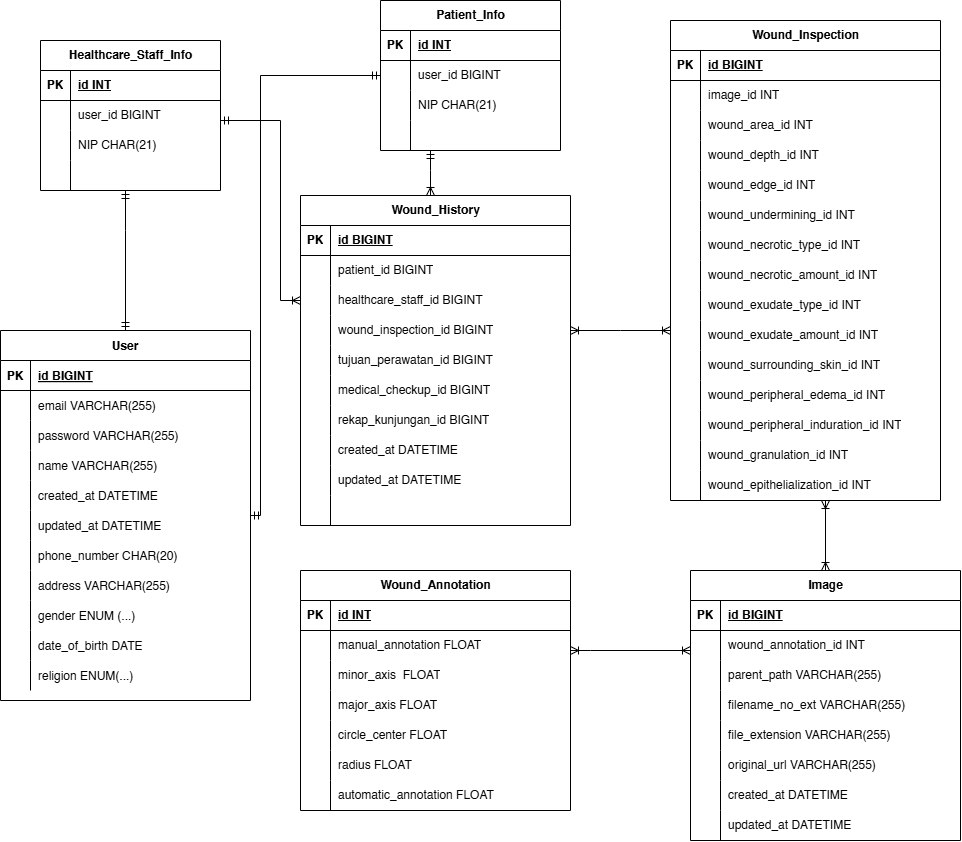
\includegraphics[keepaspectratio, width=8cm]{gambar/erd_sprint_5}
		\caption{ERD \textit{Sprint-5}}
		\label{gambar:erd_sprint_5}
	\end{figure}
\end{enumerate}

\subsection{\textit{Sprint 6}}
\textit{Sprint-6} ini terdapat 1 \textit{story} yaitu membuat fitur \textit{wound history}. \textit{Story} tersebut diurai menjadi beberapa bagian sebagai berikut.
	\begin{table}[H]
	\caption{\textit{Sprint 6}}
	\label{sprint6_backlog}
	\begin{tabular}{@{} |p{0.5cm}|p{5cm}|p{5cm}|p{2cm}| @{}}
		\hline
		\textbf{No.} & \textbf{\textit{User Story}} & \textbf{\textit{Task}} & \textbf{\textit{Status}} \\
		\hline
		\multirow{3}{3cm}{1.} & \multirow{3}{5cm}{\textit{Wound History}} & Analisis dan Perancangan Wound History & selesai\\
		\cline{3-4}
		 & & Implementasi Backend untuk Wound History & selesai\\
		\cline{3-4}
		& & Implementasi Frontend untuk Wound History & selesai\\
		\hline
	\end{tabular}
	\end{table}
Pada \textit{sprint} ini membuat fitur \textit{wound history}. Tujuannya agar dapat memantau perkembangan penyembuhan dan menentukan tindakan perawatan yang tepat.
\begin{enumerate}
\item Analisis dan Perancangan Wound History

Menganalisis data yang diperlukan dalam riwayat luka. Mendesain struktur database untuk menyimpan data riwayat luka. Membuat alur riwayat luka pasien.
	\begin{figure}[H]
		\centering
		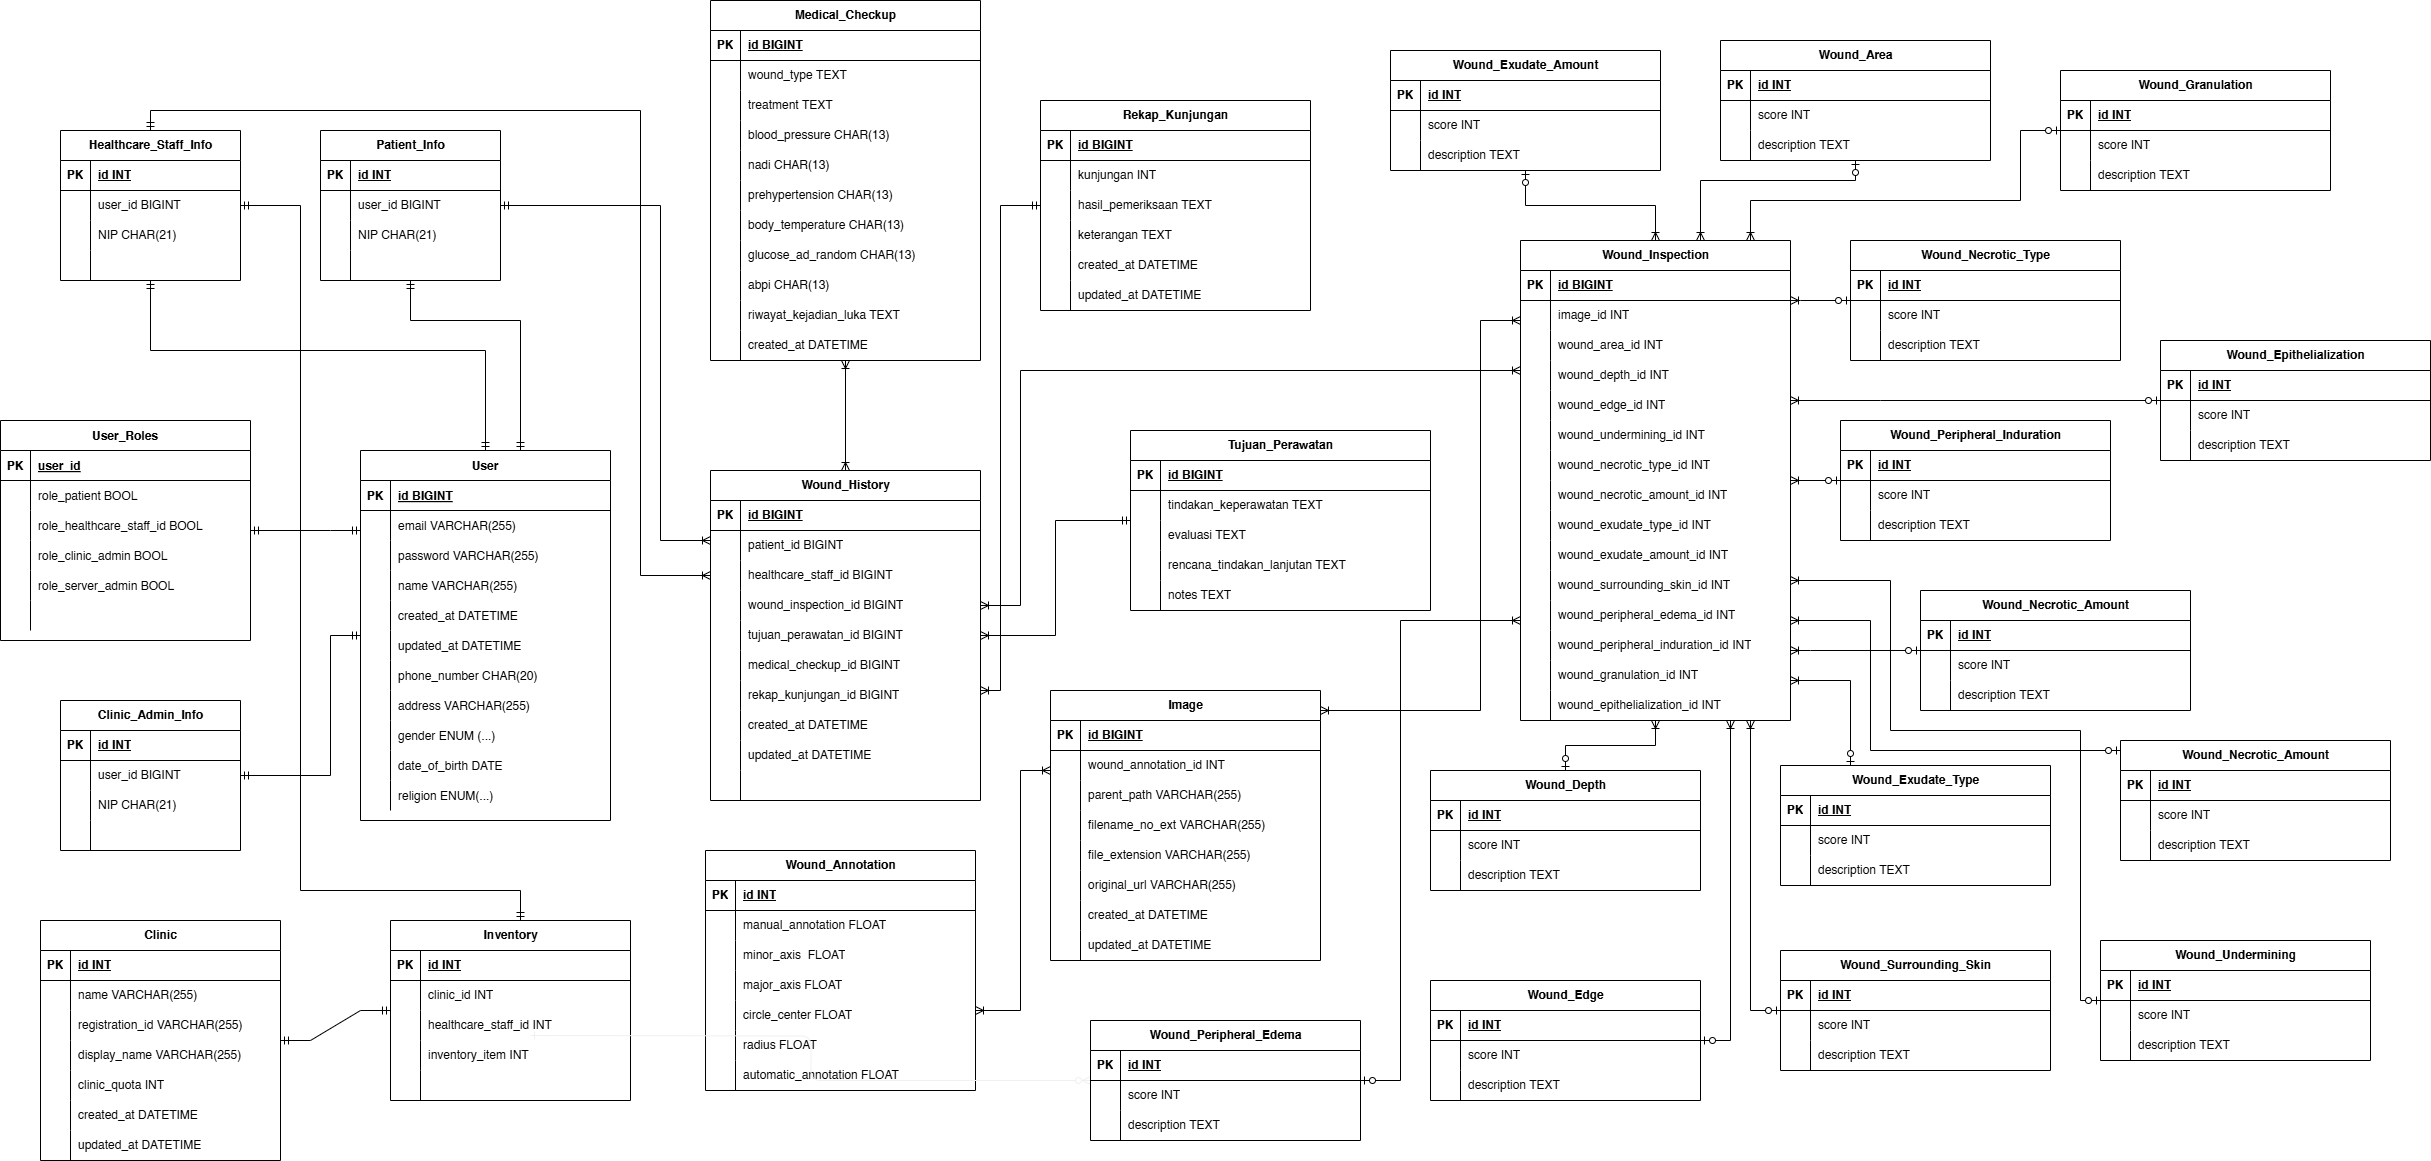
\includegraphics[keepaspectratio, width=10cm]{gambar/erd_full}
		\caption{\textit{Entity Relation Diagram} Sistem Keseluruhan}
		\label{gambar:erd_sprint_6}
	\end{figure}
	\begin{figure}[H]
		\centering
		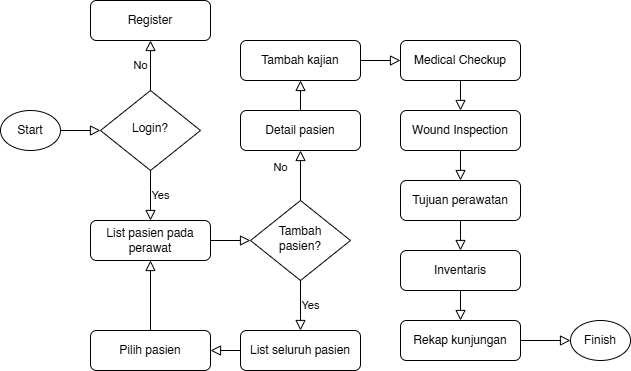
\includegraphics[keepaspectratio, width=8cm]{gambar/flowchart_wound_history}
		\caption{\textit{Flowchart Wound History}}
		\label{gambar:flowchart_wound_history}
	\end{figure}
\item Implementasi Backend untuk Wound History

Membuat API untuk mengambil dan menyimpan data riwayat luka. Lalu menghubungkan API dengan database sistem.
\textit{Implementasi Backend}
\begin{lstlisting}
@bp.route("v1/wound_history/", methods=["POST"])
def create_wound_history():
    try:
        return json.dumps({"message" : str(db_histori_kajian.create_wound_history(request)) })
    except Exception as ex:
        print(ex)
        return Response(response = json.dumps({"message" : f"{ex}"}), mimetype="application/json", status=500)
    
@bp.route("v1/wound_history/patient/<patient_id>", methods=["GET"])
def get_all_wound_history_by_patient_id(patient_id):
    try:
        return db_histori_kajian.get_all_wound_history_by_patient_id(patient_id)
    except Exception as ex:
        print(ex)
        return Response(response = json.dumps({"message" : f"{ex}"}), mimetype="application/json", status=500)
\end{lstlisting}
\item Implementasi Frontend untuk Wound History

Mengembangkan tampilan riwayat luka pasien pada aplikasi, menampilkan daftar riwayat luka, serta mengintegrasikan frontend dengan API yang telah dibuat.
\begin{lstlisting}
    @GET("v1/wound_history/patient/{patient_id}")
    suspend fun getAllWoundHistory(
        @Path("patient_id") patient_id: String
    ): Response<Collection<WoundHistoryItem>>

    @GET("v1/wound_history/{wound_history_id}")
    suspend fun getDetailWoundHistory(
        @Path("wound_history_id") wound_history_id: String
    ): Response<DetailWoundHistory>
\end{lstlisting}
\end{enumerate}

\subsection{\textit{Sprint 7}}
Pada \textit{Sprint-7} ini terdapat 4 \textit{story} yang berfokus pada fitur pengembangan pasien sebagai berikut.
	\begin{table}[H]
	\caption{\textit{Sprint 7}}
	\label{sprint7_backlog}
	\begin{tabular}{@{} |p{0.5cm}|p{5cm}|p{5cm}|p{2cm}| @{}}
		\hline
		\textbf{No.} & \textbf{\textit{User Story}} & \textbf{\textit{Task}} & \textbf{\textit{Status}} \\
		\hline
		\multirow{3}{3cm}{1.} & \multirow{3}{5cm}{Registrasi akun pasien} & Analisis kebutuhan dan perancangan fitur registrasi. & selesai\\
		\cline{3-4}
		 & & Implementasi backend API untuk menangani registrasi & selesai\\
		\cline{3-4}
		& & Implementasi frontend untuk formulir registrasi dengan validasi input & selesai\\
		\hline
		\multirow{3}{3cm}{1.} & \multirow{3}{5cm}{Mengambil nomor antrean} & Desain UI untuk tampilan pemilihan layanan dan nomor antrean. & selesai\\
		\cline{3-4}
		 & & Integrasi web service backend API untuk pemrosesan antrean pasien & tidak selesai\\
		\cline{3-4}
		 & & Pengembangan frontend untuk mengambil dan menampilkan nomor antrean & tidak selesai\\
		\hline
		\multirow{3}{3cm}{1.} & \multirow{3}{5cm}{Pasien melihat rekap kunjungan} & Merancang tampilan daftar kunjungan & selesai\\
		\cline{3-4}
		 & & Implementasi backend API untuk mengambil data riwayat kunjungan pasien & selesai\\
		\cline{3-4}
		 & & Pengembangan frontend untuk menampilkan riwayat kunjungan dalam format yang mudah dibaca & selesai\\
		\hline
		\multirow{3}{3cm}{1.} & \multirow{3}{5cm}{Pasien melihat riwayat kajian luka} & Desain tampilan daftar riwayat kajian luka untuk pasien. & selesai\\
		\cline{3-4}
		 & & Pengembangan frontend untuk menampilkan riwayat kajian luka & selesai\\
		\hline
	\end{tabular}
	\end{table}
\textit{Sprint} ini berfokus pada pengalaman pasien dalam mengakses layanan digital klinik, dari registrasi, antrean, hingga melihat riwayat perawatan mereka. Kendala yang dialami oleh penulis adalah tidak bisanya integrasi dengan web service antrean klinik dikarenakan pada penelitian sebelumnya tidak selesai.
\begin{enumerate}
\item Analisis kebutuhan dan perancangan fitur registrasi

Membuat rancangan model fitur register pasien. Dilanjutkan dengan membuat tampilan yang telah dikembangkan berdasarkan rancangan model.
	\begin{figure}[H]
		\centering
		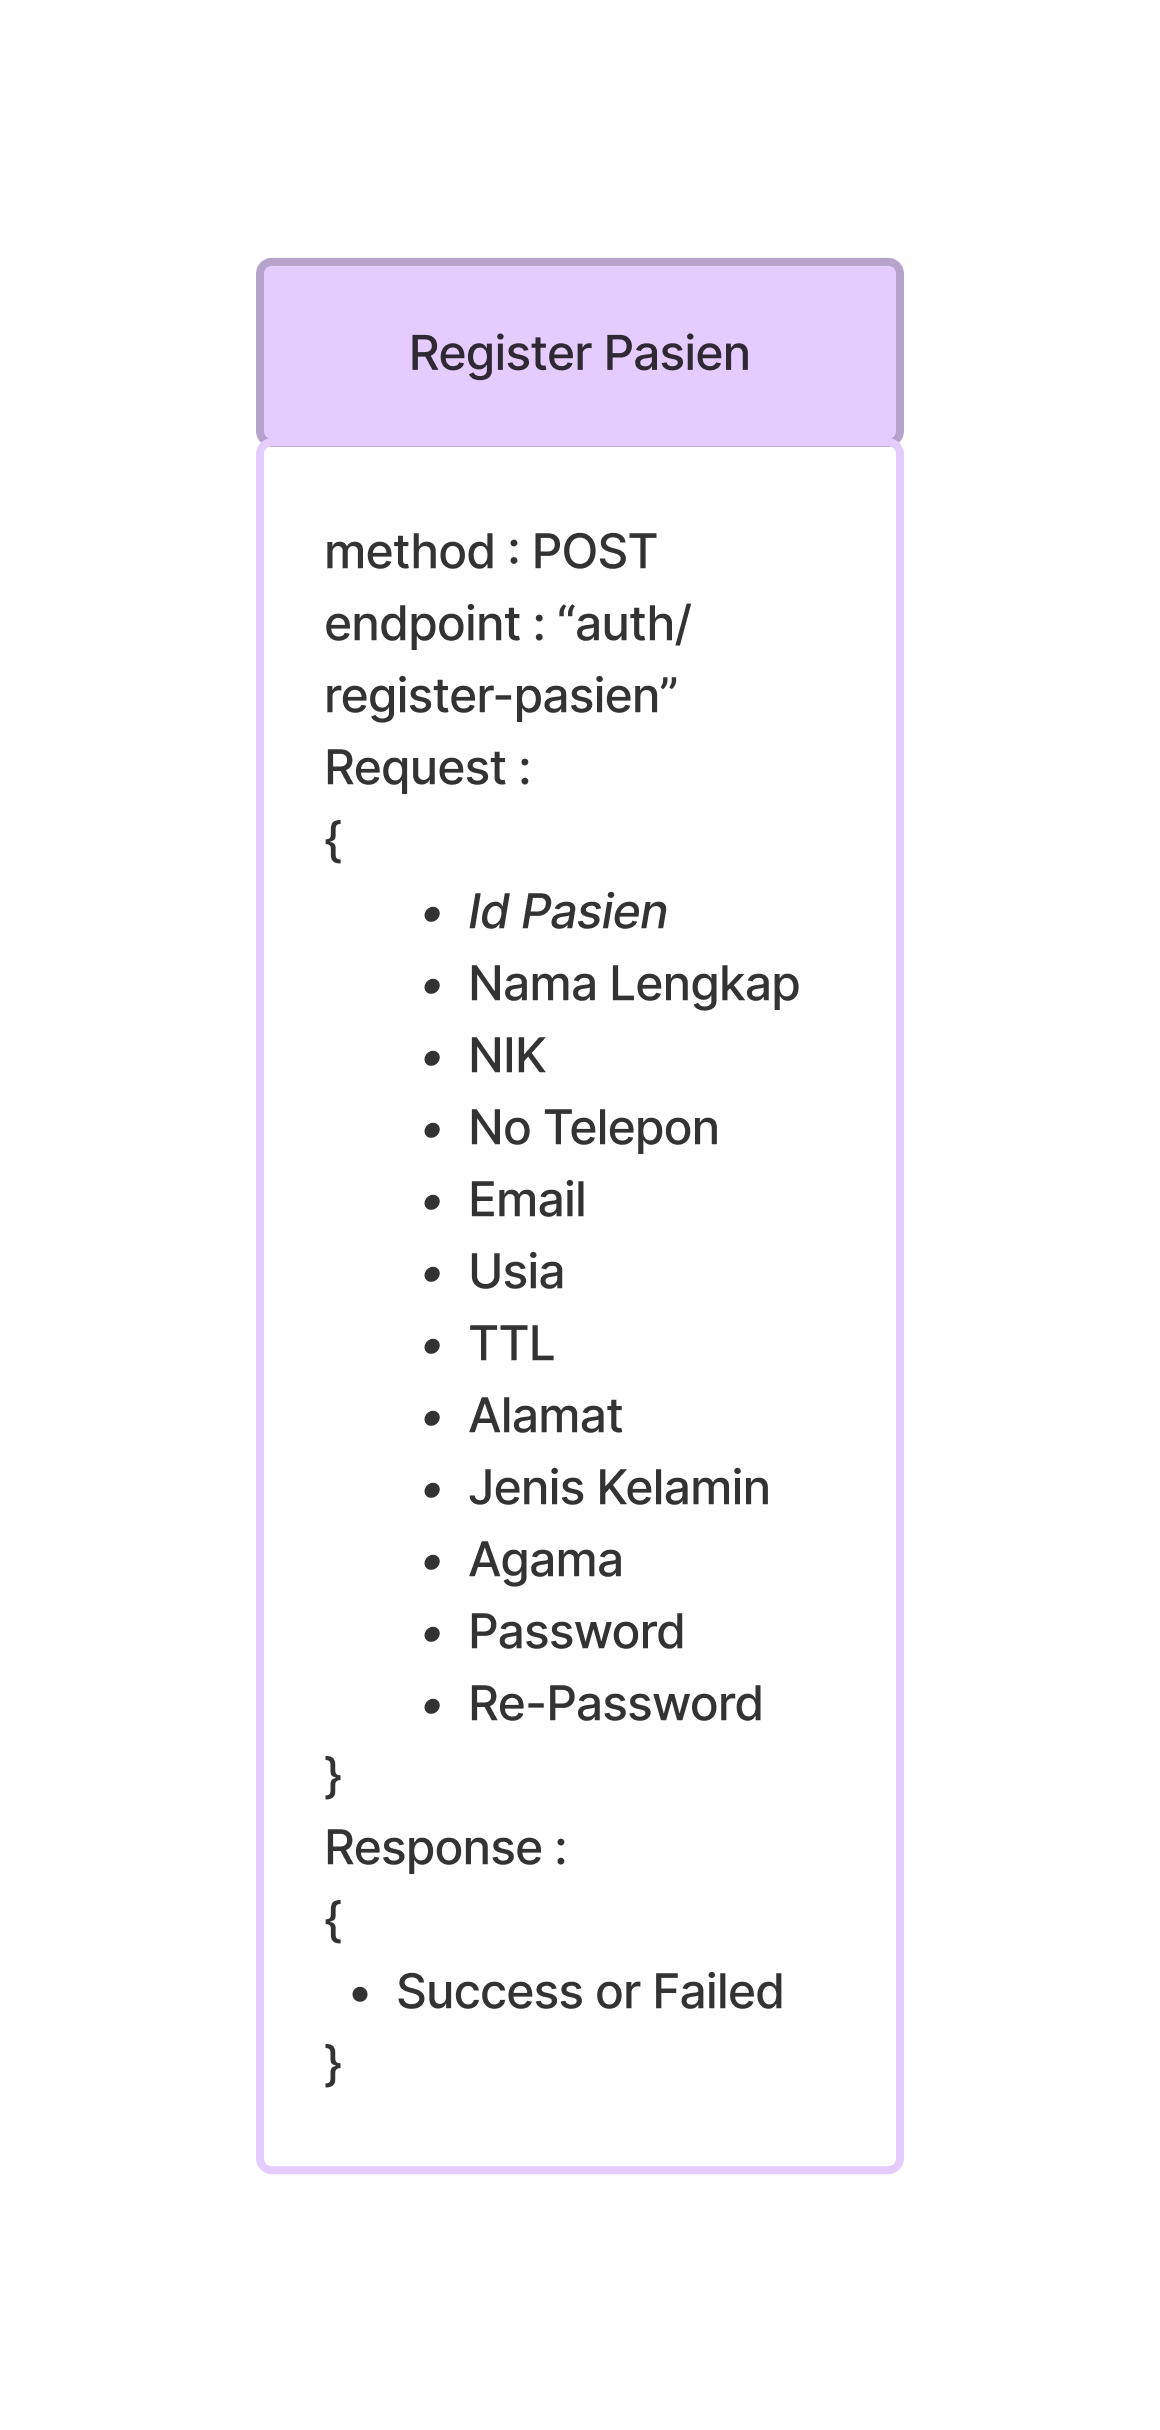
\includegraphics[keepaspectratio, width=3cm]{gambar/rancangan_fitur_registrasi}
		\caption{\textit{Flowchart Wound History}}
		\label{gambar:rancangan_fitur_registrasi}
	\end{figure}
	\begin{figure}[H]
		\centering
		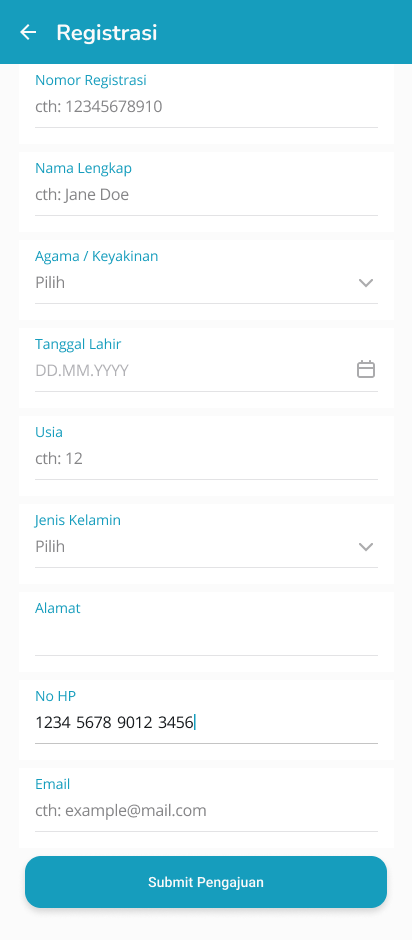
\includegraphics[keepaspectratio, width=4cm]{gambar/tampilan_registrasi}
		\caption{Desain tampilan registrasi pasien}
		\label{gambar:tampilan_registrasi}
	\end{figure}
\item Implementasi backend API untuk menangani registrasi

Implementasi yang dilakukan seperti halnya dengan register user baru dengan tambahan \textit{roles} untuk membedakan pasien dan perawat.

\begin{lstlisting}
@bp.route("v1/patient", methods=["POST"])
def create_patient():
    try:
        return json.dumps({"message" : db_user_new.create_patient(request) })
    except Exception as ex:
        print(ex)
        return Response(response = json.dumps({"message" : f"{ex}"}), mimetype="application/json", status=500)

def create_patient(request):
    data = {
        "email": request.form["email"],
        "password": request.form["password"],
        "updated_at": time.strftime("%d/%m/%Y %H:%M:%S"),
        "created_at": time.strftime("%d/%m/%Y %H:%M:%S"),
    }
    if request.form.get("registration_id")!='""' and request.form.get("registration_id")!="" and request.form.get("registration_id")!="''" and request.form.get("registration_id")!=None:
        pass
    else:
        raise Exception("id registrasi tidak ada")
    check = get_from_collection("user",{"email":request.form["email"]})
    check = json.loads(bson.json_util.dumps(list(check)))
    if len(check) !=0:
        raise Exception("email yang dimasukkan telah digunakan")
    nullable = {"name":"string","phone_number": "string","address":"string","gender":"string","religion":"string","date_of_birth":"date"}
    for param in nullable.keys():
        if request.form.get(param)!='""' and request.form.get(param)!="" and request.form.get(param)!="''" and request.form.get(param)!=None:
            if nullable[param]=="string":
                data[param] = request.form[param]
            elif nullable[param]=="int":
                data[param] = int(request.form[param])
            elif nullable[param]=="date":
                data[param] = request.form[param]
        else:
            data[param] = None
    user_id = insert_to_collection("user",data).inserted_id
    data = {
        "user_id": user_id,
        "role_patient" : True,
        "role_healthcare_staff": False,
        "role_clinic_admin": False,
        "role_server_admin": False,
    }
    insert_to_collection("user_roles", data)
    data = {
        "user_id": user_id,
        "registration_id": request.form["registration_id"],
        "healthcare_staff_id": [],
        }
    insert_to_collection("patient_info", data)
    return "Berhasil menambahkan pasien baru"
\end{lstlisting}
\item Implementasi frontend untuk formulir registrasi dengan validasi input

	\begin{figure}[H]
		\centering
		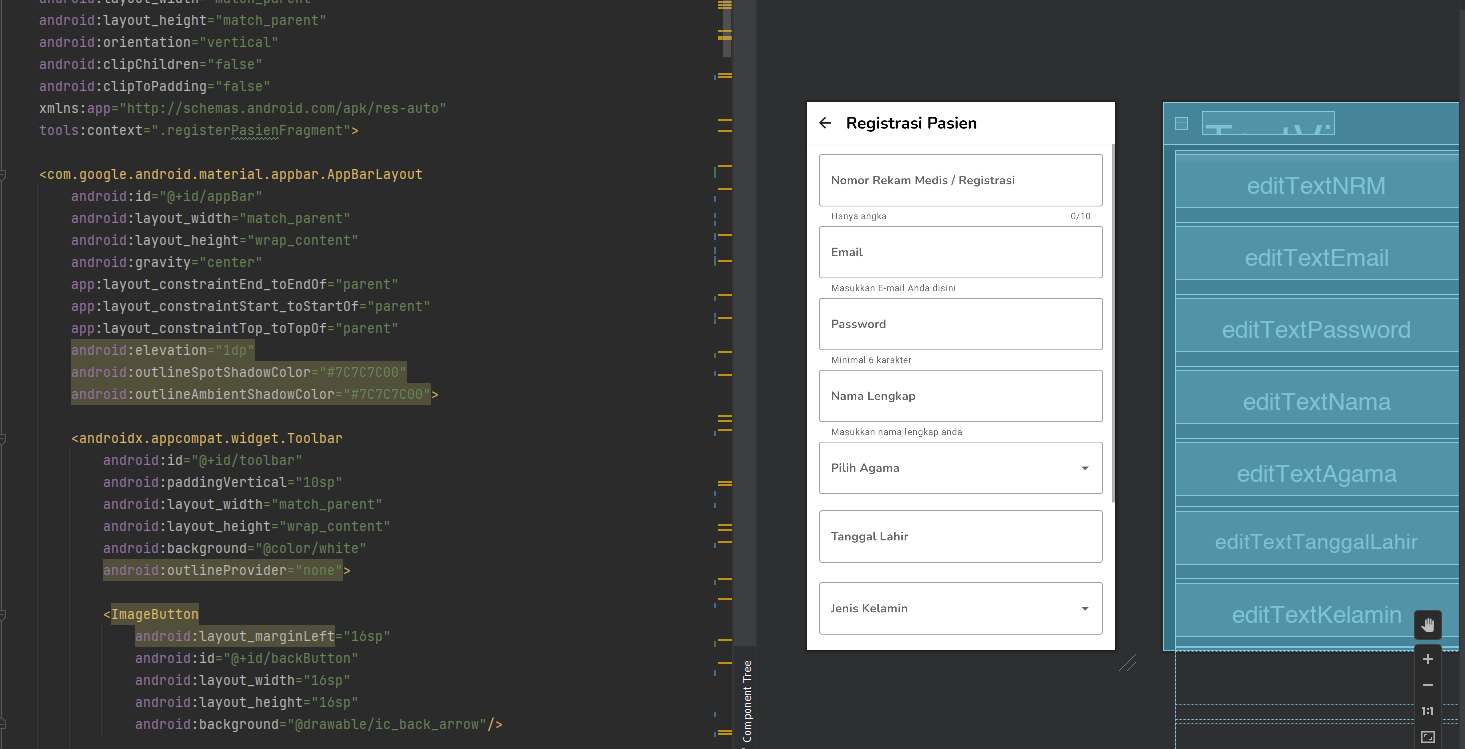
\includegraphics[keepaspectratio, width=10cm]{gambar/fragment_registrasi_pasien}
		\caption{Fragment registrasi pasien}
		\label{gambar:fragment_registrasi_pasien}
	\end{figure}

\item Desain UI untuk tampilan mengambil nomor antrean

	\begin{figure}[H]
		\centering
		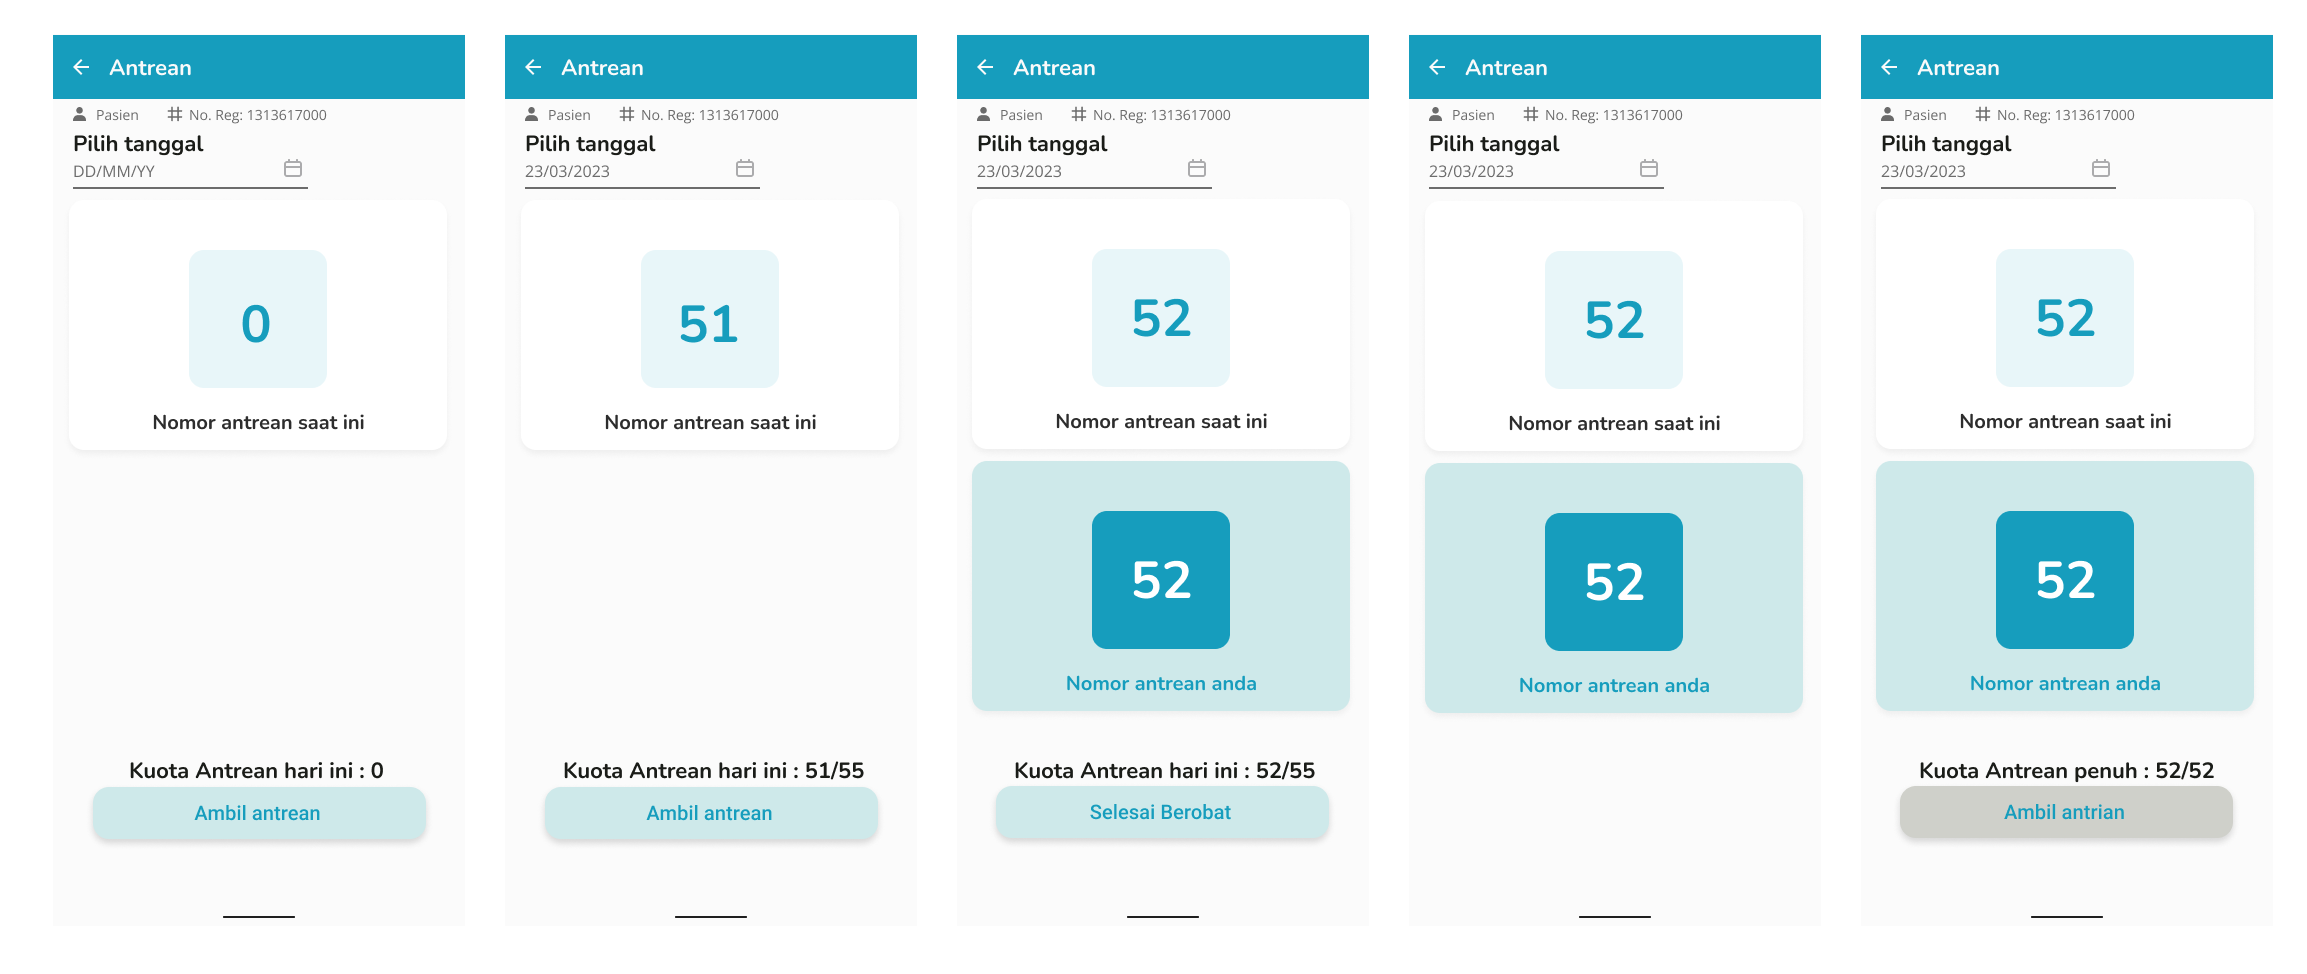
\includegraphics[keepaspectratio, width=12cm]{gambar/tampilan_antrean}
		\caption{Fragment registrasi pasien}
		\label{gambar:tampilan_antrean}
	\end{figure}

\item Integrasi web service backend API untuk pemrosesan antrean pasien

Kendala yang dialami oleh penulis adalah belum selesainya web service klinik pada penelitian sebelumnya yang mengakibatkan tidak dapat dilanjutkannya integrasi web service untuk antrean.
\item Merancang tampilan daftar kunjungan

Desain tampilannya sama dengan yang ada pada fitur rekap kunjungan di perawat. Pasien juga dapat menggunakannya.
\item Implementasi backend API untuk mengambil data riwayat kunjungan pasien

\textit{Implementasi backend}
\begin{lstlisting}
@bp.route("v1/rekap_kunjungan/<id_rekap_kunjungan>", methods=["GET"])
def get_rekap_kunjungan_by_id(id_rekap_kunjungan):
    try:
        return db_rekap_kunjungan.get_rekap_kunjungan_by_id(id_rekap_kunjungan)
    except Exception as ex:
        print(ex)
        return Response(response = json.dumps({"message" : f"{ex}"}), mimetype="application/json", status=500)
    
@bp.route("v1/rekap_kunjungan/patient/<patient_id>", methods=["GET"])
def get_rekap_kunjungan_by_patient_id(patient_id):
    try:
        return db_rekap_kunjungan.get_rekap_kunjungan_by_patient_id(patient_id)
    except Exception as ex:
        print(ex)
        return Response(response = json.dumps({"message" : f"{ex}"}), mimetype="application/json", status=500)
\end{lstlisting}
\item Pengembangan frontend untuk menampilkan riwayat kunjungan dalam format yang mudah dibaca

Sama seperti tampilan yang terdapat dalam fitur rekap kunjungan pada perawat. Perbedaanya hanyalah pada beberapa spesifik \textit{field} yang tidak ditampilkan.

\item Desain tampilan daftar riwayat kajian luka untuk pasien

	\begin{figure}[H]
		\centering
		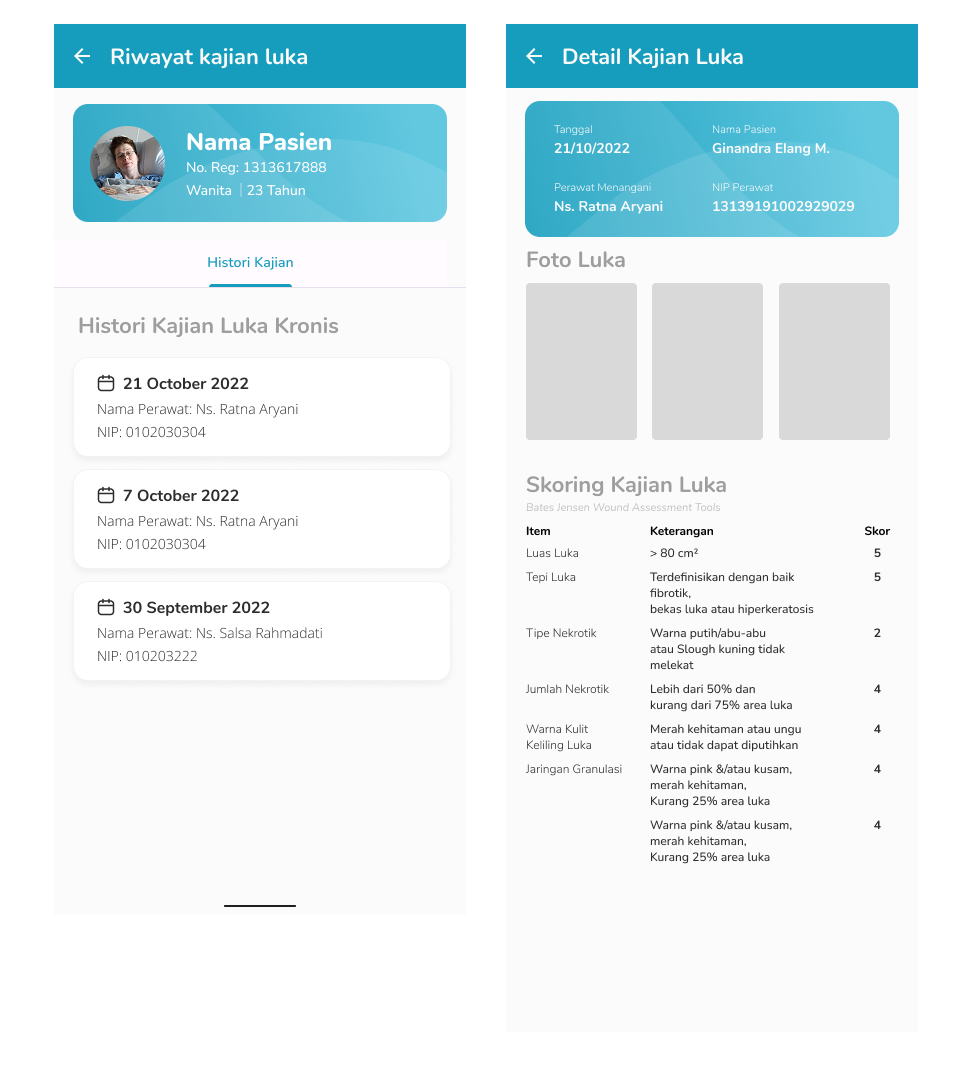
\includegraphics[keepaspectratio, width=12cm]{gambar/tampilan_riwayat_luka}
		\caption{Tampilan riwayat luka}
		\label{gambar:tampilan_riwayat_luka}
	\end{figure}
\item Pengembangan frontend untuk menampilkan riwayat kajian luka

Sama seperti tampilan yang dilihat oleh fitur \textit{wound history} perawat. Tetapi perbedaannya hanya beberapa \textit{field} saja yang ditampilkan.
\end{enumerate}

\subsection{\textit{Sprint 8}}
\textit{Sprint-8} ini berisi 1 \textit{story} yaitu membuat fitur inventaris. \textit{Story} tersebut dapat diuraikan lagi menjadi sebagai berikut.
	\begin{table}[H]
	\caption{\textit{Sprint 8}}
	\label{sprint8_backlog}
	\begin{tabular}{@{} |p{0.5cm}|p{5cm}|p{5cm}|p{2cm}| @{}}
		\hline
		\textbf{No.} & \textbf{\textit{User Story}} & \textbf{\textit{Task}} & \textbf{\textit{Status}} \\
		\hline
		\multirow{3}{3cm}{1.} & \multirow{3}{5cm}{Inventaris} & UI Design & selesai\\
		\cline{3-4}
		 & & Pengembangan struktur database & selesai\\
		\cline{3-4}
		& & Endpoint API pada fitur inventaris & selesai\\
		\cline{3-4}
		 & & Pengembangan frontend inventaris & selesai\\
		\cline{3-4}
		\hline
	\end{tabular}
	\end{table}
Tujuan dari \textit{sprint-8} adalah untuk mengelola inventaris alat medis dan obat-obatan agar ketersediaan peralatan yang dibutuhkan dalam perawatan pasien dapat dipastikan. Dalam hal ini pengembangan struktur database, membuat \textit{Endpoint API} pada fitur inventaris, dan pengembangan frontend inventaris.

\begin{enumerate}
\item \textit{UI Design}

Membuat tampilan daftar inventaris yang mudah diakses oleh perawat.
	\begin{figure}[H]
		\centering
		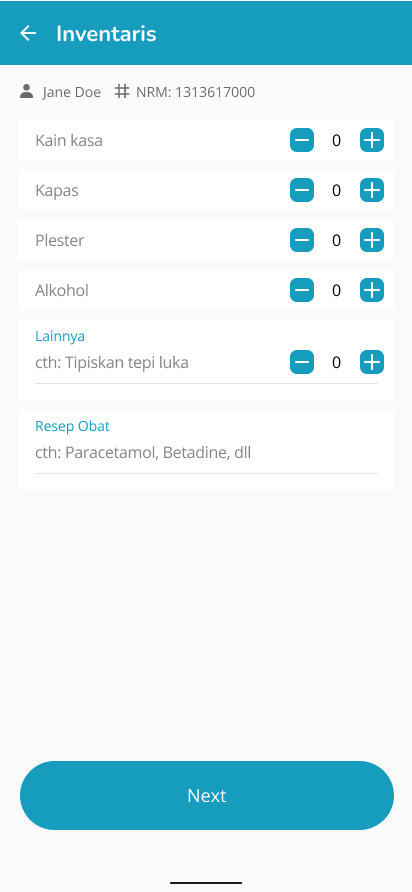
\includegraphics[keepaspectratio, width=4cm]{gambar/tampilan_inventaris}
		\caption{Tampilan inventaris}
		\label{gambar:tampilan_inventaris}
	\end{figure}
\item Pengembangan struktur database

Berikut adalah rancangan ERD terkait fitur inventaris yang sedang dikembangkan.
	\begin{figure}[H]
		\centering
		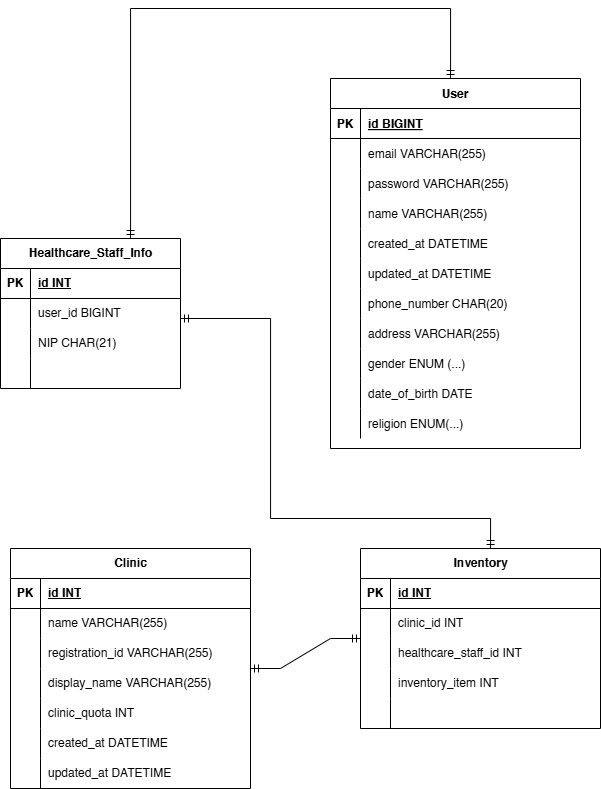
\includegraphics[keepaspectratio, width=4cm]{gambar/erd_sprint_8}
		\caption{\textit{ERD Sprint-8}}
		\label{gambar:erd_sprint_8}
	\end{figure}
\item Endpoint API pada fitur inventaris

Implementasi pada backend untuk membuat endpoint API menambahkan, memperbarui, dan menghapus data inventaris. 
\begin{lstlisting}
e@bp.route("v1/inventaris/", methods=["POST"])
def create_inventaris():
    try:
        return json.dumps({"inventaris_id" : str(db_inventaris.create_inventaris(request)) })
    except Exception as ex:
        print(ex)
        return Response(response = json.dumps({"message" : f"{ex}"}), mimetype="application/json", status=500)
    
@bp.route("v1/inventaris/<id_inventaris>", methods=["GET"])
def get_inventaris_by_id(id_inventaris):
    try:
        return db_inventaris.get_inventaris_by_id(id_inventaris)
    except Exception as ex:
        print(ex)
        return Response(response = json.dumps({"message" : f"{ex}"}), mimetype="application/json", status=500)
\end{lstlisting}

\item Pengembangan frontend inventaris

Membuat tampilan daftar inventaris sebelumnya yang mudah diakses oleh perawat kedalam bentuk fragment.
\begin{lstlisting}
class InventarisFragment : Fragment() {
    private var _binding: FragmentInventarisBinding? = null
    private val binding get() = _binding!!

    override fun onCreateView(
        inflater: LayoutInflater, container: ViewGroup?, savedInstanceState: Bundle?
    ): View {
        _binding = FragmentInventarisBinding.inflate(inflater, container, false)
        return binding.root
    }

    override fun onViewCreated(view: View, savedInstanceState: Bundle?) {
        super.onViewCreated(view, savedInstanceState)

        // Setup counter for each inventory item
        setupCounter(binding.imageButtonAddKainKasa, binding.imageButtonMinusKainKasa, binding.editTextNumberKainKasa)
        setupCounter(binding.imageButtonAddKapas, binding.imageButtonMinusKapas, binding.editTextNumberKapas)
        setupCounter(binding.imageButtonAddPlester, binding.imageButtonMinusPlester, binding.editTextNumberPlester)
        setupCounter(binding.imageButtonAddAlkohol, binding.imageButtonMinusAlkohol, binding.editTextNumberAlkohol)
        setupCounter(binding.imageButtonAddInventarisLainnya, binding.imageButtonMinusInventarisLainnya, binding.editTextNumberInventarisLainnya)

        binding.buttonSubmit.setOnClickListener {
            sendDataToServer()
        }
    }

    private fun setupCounter(addButton: ImageButton, minusButton: ImageButton, editText: EditText) {
        addButton.setOnClickListener {
            val value = editText.text.toString().toIntOrNull() ?: 0
            if (value < 99) editText.setText((value + 1).toString())
        }

        minusButton.setOnClickListener {
            val value = editText.text.toString().toIntOrNull() ?: 0
            if (value > 0) editText.setText((value - 1).toString())
        }
    }

    private fun sendDataToServer() {
        val kainKasa = binding.editTextNumberKainKasa.text.toString()
        val kapas = binding.editTextNumberKapas.text.toString()
        val plester = binding.editTextNumberPlester.text.toString()
        val alkohol = binding.editTextNumberAlkohol.text.toString()
        val lainnya = binding.editTextNumberInventarisLainnya.text.toString()
        val resepObat = binding.editTextResepObat.text.toString()

        val action = InventarisFragmentDirections.actionInventarisFragmentToRekapKunjunganFragment()
        findNavController().navigate(action)
    }

    override fun onDestroyView() {
        super.onDestroyView()
        _binding = null
    }
}
\end{lstlisting}

\end{enumerate}

\subsection{\textit{Sprint 9}}
Pada \textit{Sprint} ini terdapat 1 \textit{story} yang berisi tentang fitur menambah pasien ke dalam akun perawat. \textit{Story} tersebut diurai menjadi beberapa bagian sebagai berikut.
	\begin{table}[H]
	\caption{\textit{Sprint 9}}
	\label{sprint9_backlog}
	\begin{tabular}{@{} |p{0.5cm}|p{5cm}|p{5cm}|p{2cm}| @{}}
		\hline
		\textbf{No.} & \textbf{\textit{User Story}} & \textbf{\textit{Task}} & \textbf{\textit{Status}} \\
		\hline
		\multirow{3}{3cm}{1.} & \multirow{3}{5cm}{Menambah pasien ke dalam akun perawat} & UI Design & selesai\\
		\cline{3-4}
		 & & Pengembangan backend & selesai\\
		\cline{3-4}
		& & Pengembangan frontend berdasarkan desain & selesai\\
		\cline{3-4}
		\hline
	\end{tabular}
	\end{table}
Tujuan dari \textit{sprint} ini adalah dapat menambahkan pasien ke dalam akun perawat agar perawat bisa melihat daftar pasien yang pernah ditangani dan memantau perkembangan perawatan. Kendala yang penulis alami pada \textit{sprint} kali ini adalah proses pengembangan backend.
\begin{enumerate}
\item \textit{UI Design}

Mengumpulkan kebutuhan terkait pencatatan pasien yang pernah ditangani berdasar kartu kunjungan klinik pada lampiran C. Menentukan data pasien yang akan ditampilkan dalam akun perawat (nama, NRM, riwayat perawatan, dsb.).
	\begin{figure}[H]
		\centering
		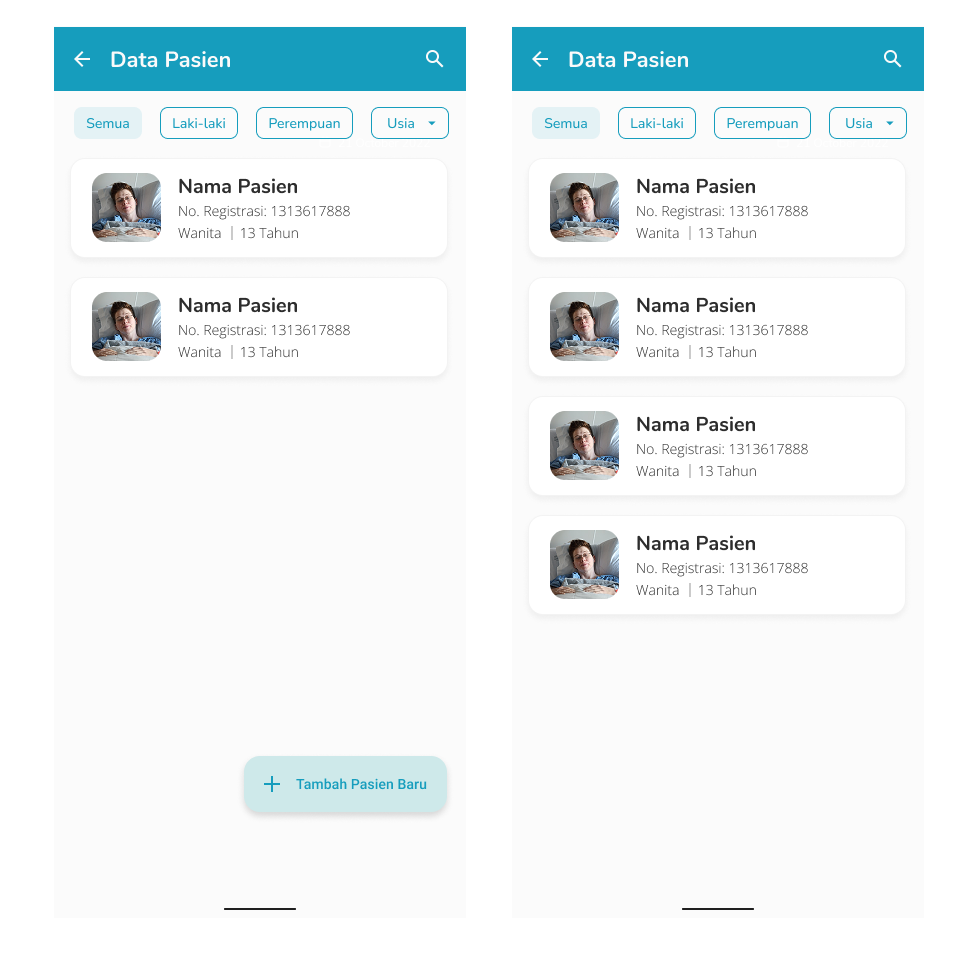
\includegraphics[keepaspectratio, width=4cm]{gambar/tampilan_data_pasien}
		\caption{\textit{UI Design Sprint-9} }
		\label{gambar:tampilan_data_pasien}
	\end{figure}
\item Pengembangan backend

Membuat endpoint API untuk menambahkan pasien ke dalam daftar akun perawat. Mengembangkan fitur untuk menghubungkan pasien dengan akun perawat berdasarkan sesi perawatan. Menyediakan fitur untuk memperbarui daftar pasien dalam akun perawat jika diperlukan.
\textit{Endpoint API}
\begin{lstlisting}
@bp.route("v1/healthcare_staff/patient",methods=["PUT"])
def insert_patient_to_healthcare_staff():
    try:
        return json.dumps({"message" : db_user_new.insert_patient_to_healthcare_staff(request) })
    except Exception as ex:
        print(ex)
        return Response(response = json.dumps({"message" : f"{ex}"}), mimetype="application/json", status=500)
\end{lstlisting}
\textit{Menghubungkan pasien dengan akun perawat}
\begin{lstlisting}
def insert_patient_to_healthcare_staff(reqeust):
    patient = get_from_collection("user", {"_id": ObjectId(reqeust.form["patient_id"])})
    patient = json.loads(bson.json_util.dumps(list(patient)))
    if len(patient) == 0:
        raise Exception(f"pasien dengan id pasien {reqeust.form['patient_id']} tidak ditemukan")
    patient = patient[0]
    healthcare_staff = get_from_collection("user", {"_id": ObjectId(reqeust.form["healthcare_staff_id"])})
    healthcare_staff = json.loads(bson.json_util.dumps(list(healthcare_staff)))
    if len(healthcare_staff) == 0:
        raise Exception(f"perawat dengan id perawat {reqeust.form['healthcare_staff_id']} tidak ditemukan")
    healthcare_staff = healthcare_staff[0]
    patient_info = get_from_collection("patient_info", {"user_id": ObjectId(patient["_id"]["$oid"])})
    patient_info = json.loads(bson.json_util.dumps(list(patient_info)))
    if len(patient_info) == 0:
        raise Exception(f"user dengan id pasien {reqeust.form['patient_id']} bukan pasien")
    patient_info = patient_info[0]
    healthcare_staff_info = get_from_collection("healthcare_staff_info", {"user_id": ObjectId(healthcare_staff["_id"]["$oid"])})
    healthcare_staff_info = json.loads(bson.json_util.dumps(list(healthcare_staff_info)))
    if len(healthcare_staff_info) == 0:
        raise Exception(f"user dengan id perawat {reqeust.form['healthcare_staff_id']} bukan perawat")
    healthcare_staff_info = healthcare_staff_info[0]
    patient_info["healthcare_staff_id"] = [
        ObjectId(item["$oid"]) if isinstance(item, dict) and "$oid" in item else ObjectId(item)
        for item in patient_info["healthcare_staff_id"]
    ]
    patient_info["healthcare_staff_id"].append(ObjectId(reqeust.form["healthcare_staff_id"]))
    healthcare_staff_info["patient_id"] = [
        ObjectId(item["$oid"]) if isinstance(item, dict) and "$oid" in item else ObjectId(item)
        for item in healthcare_staff_info["patient_id"]
    ]
    healthcare_staff_info["patient_id"].append(ObjectId(reqeust.form["patient_id"]))
    update_from_collection("patient_info", patient_info["_id"]["$oid"], {"healthcare_staff_id": patient_info["healthcare_staff_id"]})
    update_from_collection("healthcare_staff_info", healthcare_staff_info["_id"]["$oid"], {"patient_id": healthcare_staff_info["patient_id"]})

    return "Berhasil menambah pasien ke list perawat"
\end{lstlisting}
\item Pengembangan frontend berdasarkan desain

Membuat tampilan fragment daftar pasien dalam akun perawat agar mempermudah akses perawat terhadap pasien yang pernah dirawat.
	\begin{figure}[H]
		\centering
		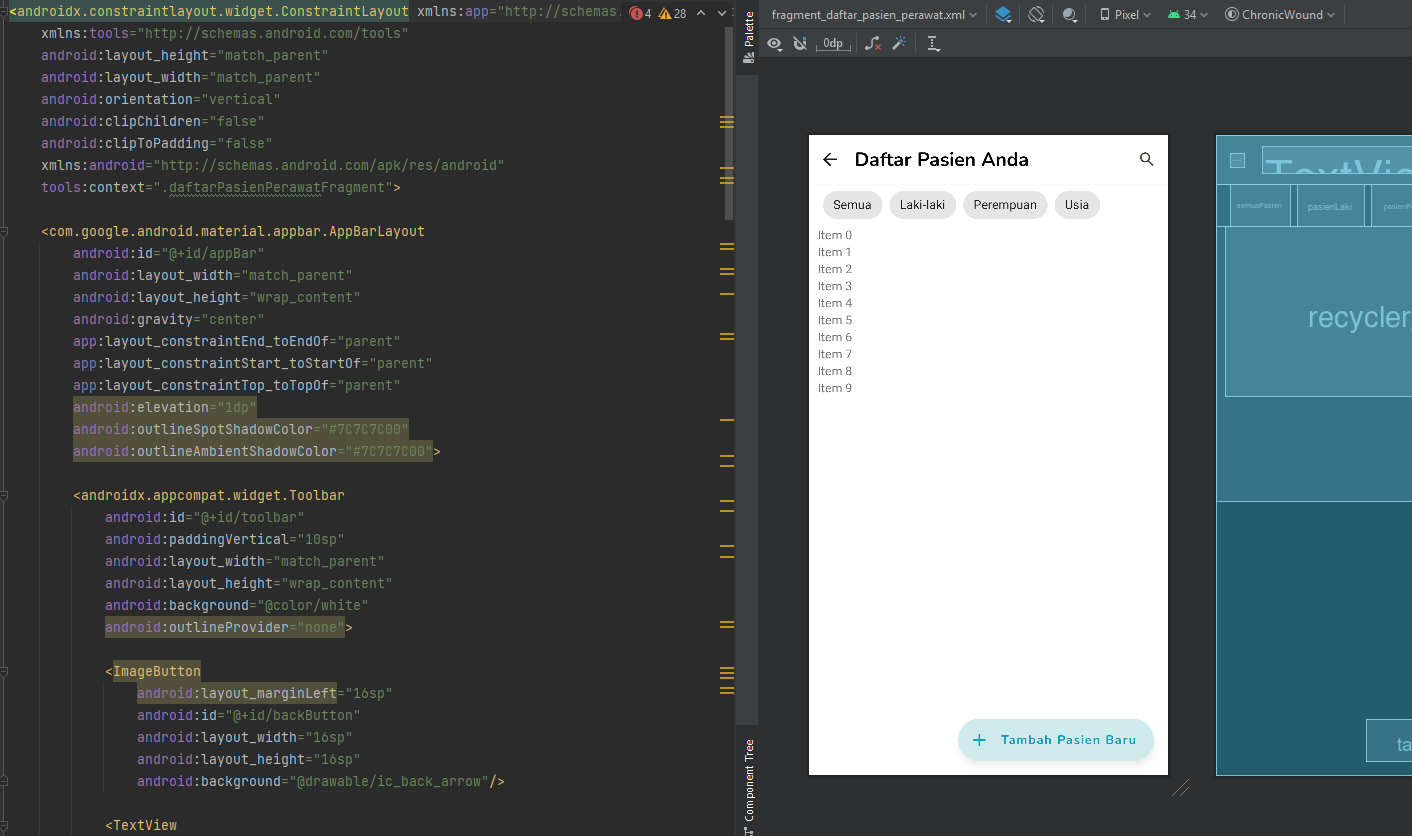
\includegraphics[keepaspectratio, width=10cm]{gambar/fragment_daftar_pasien}
		\caption{Fragment daftar pasien}
		\label{gambar:fragment_daftar_pasien}
	\end{figure}

\end{enumerate}
\section{Hasil Pengujian}
Pengujian aplikasi dilakukan melalui dua jenis metode, yaitu \textit{Unit Testing} dan User Acceptance Test (UAT). Pengujian ini dilaksanakan setelah seluruh User Story dalam Product Backlog berhasil diimplementasikan. Unit Testing dilakukan oleh satu pengembang internal, sementara User Acceptance Test dilakukan oleh seorang penguji ahli atau perawat untuk memastikan kesesuaian aplikasi dengan kebutuhan pengguna.

\subsection{Unit Testing}
Hasil dari \textit{Unit Testing} yang telah disiapkan untuk satu developer internal menunjukkan bahwa pengujian dilakukan setelah suatu fitur dinyatakan selesai. Namun, pengujian ini belum dilaksanakan secara langsung, melainkan hanya menampilkan skenario pengujiannya. Secara keseluruhan, \textit{unit testing} dirancang untuk memastikan bahwa fitur yang dikembangkan dapat berfungsi dengan baik. Rincian skenario tersebut sebagai berikut.
	\begin{longtable}{| p{8cm} | c | c | l |}
    \caption{Unit Testing Halaman Awal.\label{table:unit_halaman_awal}}\\
    \hline
    \multirow{2}{*}{Skenario Pengujian} & \multicolumn{2}{l|}{Kesesuaian} & \multirow{2}{*}{Kesimpulan} \\ 
    \cline{2-3}
      & \multicolumn{1}{l|}{sesuai} & tidak sesuai & \\ 
    \hline
    \hline
    \endfirsthead
    \hline
    \multirow{2}{*}{Skenario Pengujian} & \multicolumn{2}{l|}{Kesesuaian} & \multirow{2}{*}{Kesimpulan} \\ 
    \cline{2-3}
      & \multicolumn{1}{l|}{sesuai} & tidak sesuai &  \\ 
    \hline
    \hline
    \endhead
    \hline
    \endfoot
    
    
    \hline\hline
    \endlastfoot
    Saat aplikasi dibuka akan muncul tampilan awal dengan pilihan "Login", "Buat Akun", dan "Buat Akun Pasien" & \Checkmark &  & Diterima \\ 
    \hline
    Jika tombol "Login" ditekan, guest akan masuk ke halaman Login & \Checkmark &  & Diterima \\ 
    \hline
    Jika tombol "Buat Akun" ditekan, pengguna akan masuk ke halaman register perawat & \Checkmark &  & Diterima \\ 
    \hline
    Jika tombol "Buat Akun Pasien" ditekan, pengguna akan masuk ke halaman register pasien &  \Checkmark &  & Diterima \\ 
    \hline
    \end{longtable}

	\begin{longtable}{| p{8cm} | c | c | l |}
    \caption{Unit Testing Halaman Buat Akun.\label{table:unit_testing_buat_akun}}\\
    \hline
    \multirow{2}{*}{Skenario Pengujian} & \multicolumn{2}{l|}{Kesesuaian} & \multirow{2}{*}{Kesimpulan} \\ 
    \cline{2-3}
      & \multicolumn{1}{l|}{sesuai} & tidak sesuai & \\ 
    \hline
    \hline
    \endfirsthead
    \hline
    \multirow{2}{*}{Skenario Pengujian} & \multicolumn{2}{l|}{Kesesuaian} & \multirow{2}{*}{Kesimpulan} \\ 
    \cline{2-3}
      & \multicolumn{1}{l|}{sesuai} & tidak sesuai &  \\ 
    \hline
    \hline
    \endhead
    \hline
    \endfoot
    
    
    \hline\hline
    \endlastfoot
    Ketika mengisi form registrasi dengan lengkap kemudian submit, maka akan kembali ke halaman Login & v &  & Diterima \\ 
    \hline
    Ketika mengisi form registrasi tidak lengkap kemudian submit, maka akan menampilkan pesan kesalahan untuk melengkapi data yang kosong & \Checkmark &  & Diterima \\
    \hline
    \end{longtable}
    
	\begin{longtable}{| p{8cm} | c | c | l |}
    \caption{Unit Testing Halaman Buat Akun Pasien.\label{table:unit_testing_buat_akun_pasien}}\\
    \hline
    \multirow{2}{*}{Skenario Pengujian} & \multicolumn{2}{l|}{Kesesuaian} & \multirow{2}{*}{Kesimpulan} \\ 
    \cline{2-3}
      & \multicolumn{1}{l|}{sesuai} & tidak sesuai & \\ 
    \hline
    \hline
    \endfirsthead
    \hline
    \multirow{2}{*}{Skenario Pengujian} & \multicolumn{2}{l|}{Kesesuaian} & \multirow{2}{*}{Kesimpulan} \\ 
    \cline{2-3}
      & \multicolumn{1}{l|}{sesuai} & tidak sesuai &  \\ 
    \hline
    \hline
    \endhead
    \hline
    \endfoot
    
    
    \hline\hline
    \endlastfoot
    Ketika mengisi form registrasi dengan lengkap kemudian submit, maka akan kembali ke halaman Login & \Checkmark &  & Diterima \\ 
    \hline
    Ketika mengisi form registrasi tidak lengkap kemudian submit, maka akan menampilkan pesan kesalahan untuk melengkapi data yang kosong & \Checkmark &  & Diterima \\
    \hline
    \end{longtable}
    
	\begin{longtable}{| p{8cm} | c | c | l |}
    \caption{Unit Testing Halaman Login.\label{table:unit_testing_login}}\\
    \hline
    \multirow{2}{*}{Skenario Pengujian} & \multicolumn{2}{l|}{Kesesuaian} & \multirow{2}{*}{Kesimpulan} \\ 
    \cline{2-3}
      & \multicolumn{1}{l|}{sesuai} & tidak sesuai & \\ 
    \hline
    \hline
    \endfirsthead
    \hline
    \multirow{2}{*}{Skenario Pengujian} & \multicolumn{2}{l|}{Kesesuaian} & \multirow{2}{*}{Kesimpulan} \\ 
    \cline{2-3}
      & \multicolumn{1}{l|}{sesuai} & tidak sesuai &  \\ 
    \hline
    \hline
    \endhead
    \hline
    \endfoot
    
    
    \hline\hline
    \endlastfoot
    Ketika mengisi form login dengan data yang tidak sesuai kemudian klik submit, maka akan menampilkan pesan kesalahan username atau password & v &  & Diterima \\ 
    \hline
    Ketika mengisi form login dengan data yang sesuai dengan role perawat, maka akan masuk ke halaman beranda perawat & \Checkmark &  & Diterima \\
    \hline
    Ketika mengisi form login dengan data yang sesuai dengan role pasien, maka akan masuk ke halaman beranda pasien & \Checkmark &  & Diterima \\
    \hline
    \end{longtable}
    
    \begin{longtable}{| p{8cm} | c | c | l |}
    \caption{Unit Testing Beranda Perawat.\label{table:unit_beranda_perawat}}\\
    \hline
    \multirow{2}{*}{Skenario Pengujian} & \multicolumn{2}{l|}{Kesesuaian} & \multirow{2}{*}{Kesimpulan} \\ 
    \cline{2-3}
      & \multicolumn{1}{l|}{sesuai} & tidak sesuai & \\ 
    \hline
    \hline
    \endfirsthead
    \hline
    \multirow{2}{*}{Skenario Pengujian} & \multicolumn{2}{l|}{Kesesuaian} & \multirow{2}{*}{Kesimpulan} \\ 
    \cline{2-3}
      & \multicolumn{1}{l|}{sesuai} & tidak sesuai &  \\ 
    \hline
    \hline
    \endhead
    \hline
    \endfoot
    
    
    \hline\hline
    \endlastfoot
    Saat ikon profil pada kanan atas di-klik maka akan muncul halaman profil perawat & \Checkmark &  & Diterima \\ 
    \hline
    Saat tombol daftar pasien di-klik maka akan muncul halaman daftar pasien & \Checkmark &  & Diterima \\
    \hline
    \end{longtable}
    
    \begin{longtable}{| p{8cm} | c | c | l |}
    \caption{Unit Testing Profil Perawat.\label{table:unit_profil_perawat}}\\
    \hline
    \multirow{2}{*}{Skenario Pengujian} & \multicolumn{2}{l|}{Kesesuaian} & \multirow{2}{*}{Kesimpulan} \\ 
    \cline{2-3}
      & \multicolumn{1}{l|}{sesuai} & tidak sesuai & \\ 
    \hline
    \hline
    \endfirsthead
    \hline
    \multirow{2}{*}{Skenario Pengujian} & \multicolumn{2}{l|}{Kesesuaian} & \multirow{2}{*}{Kesimpulan} \\ 
    \cline{2-3}
      & \multicolumn{1}{l|}{sesuai} & tidak sesuai &  \\ 
    \hline
    \hline
    \endhead
    \hline
    \endfoot
    
    
    \hline\hline
    \endlastfoot
    Saat halaman profil perawat muncul maka akan tampil informasi umum perawat dan tombol logout & \Checkmark &  & Diterima \\ 
    \hline
    Saat tombol logout di-klik maka akan kembali ke halaman login & \Checkmark &  & Diterima \\
    \hline
    Ketika ikon panah ke arah kiri pada kiri atas ditekan, maka akan kembali ke halaman inventaris & \Checkmark &  & Diterima \\
    \hline
    \end{longtable}
    
    \begin{longtable}{| p{8cm} | c | c | l |}
    \caption{Unit Testing Halaman Daftar Pasien.\label{table:unit_daftar_pasien}}\\
    \hline
    \multirow{2}{*}{Skenario Pengujian} & \multicolumn{2}{l|}{Kesesuaian} & \multirow{2}{*}{Kesimpulan} \\ 
    \cline{2-3}
      & \multicolumn{1}{l|}{sesuai} & tidak sesuai & \\ 
    \hline
    \hline
    \endfirsthead
    \hline
    \multirow{2}{*}{Skenario Pengujian} & \multicolumn{2}{l|}{Kesesuaian} & \multirow{2}{*}{Kesimpulan} \\ 
    \cline{2-3}
      & \multicolumn{1}{l|}{sesuai} & tidak sesuai &  \\ 
    \hline
    \hline
    \endhead
    \hline
    \endfoot
    
    
    \hline\hline
    \endlastfoot
    Saat daftar pasien dibuka, maka yang tampil hanya daftar pasien yang terdaftar pada perawat & \Checkmark &  & Diterima \\ 
    \hline
    Saat salah satu pasien dipilih maka akan muncul halaman detail pasien & \Checkmark &  & Diterima \\
    \hline
    Saat tombol tambah pasien ditekan maka akan muncul halaman daftar seluruh pasien & \Checkmark &  & Diterima \\
    \hline
    Ketika ikon panah ke arah kiri pada kiri atas ditekan, maka akan kembali ke halaman beranda perawat & \Checkmark &  & Diterima \\
    \hline
    \end{longtable}
    
    \begin{longtable}{| p{8cm} | c | c | l |}
    \caption{Unit Testing Halaman Daftar Seluruh Pasien.\label{table:unit_daftar_seluruh_pasien}}\\
    \hline
    \multirow{2}{*}{Skenario Pengujian} & \multicolumn{2}{l|}{Kesesuaian} & \multirow{2}{*}{Kesimpulan} \\ 
    \cline{2-3}
      & \multicolumn{1}{l|}{sesuai} & tidak sesuai & \\ 
    \hline
    \hline
    \endfirsthead
    \hline
    \multirow{2}{*}{Skenario Pengujian} & \multicolumn{2}{l|}{Kesesuaian} & \multirow{2}{*}{Kesimpulan} \\ 
    \cline{2-3}
      & \multicolumn{1}{l|}{sesuai} & tidak sesuai &  \\ 
    \hline
    \hline
    \endhead
    \hline
    \endfoot
    
    
    \hline\hline
    \endlastfoot
    Saat daftar seluruhpasien dibuka, maka seluruh akun pasien yang telah register akan tampil & \Checkmark &  & Diterima \\ 
    \hline
    Saat salah satu pasien dipilih maka akan muncul halaman daftar pasien & \Checkmark &  & Diterima \\
    Ketika ikon panah ke arah kiri pada kiri atas ditekan, maka akan kembali ke halaman daftar pasien & \Checkmark &  & Diterima \\
    \hline
    \end{longtable}
    
    \begin{longtable}{| p{8cm} | c | c | l |}
    \caption{Unit Testing Halaman Detail Pasien.\label{table:unit_detail_pasien}}\\
    \hline
    \multirow{2}{*}{Skenario Pengujian} & \multicolumn{2}{l|}{Kesesuaian} & \multirow{2}{*}{Kesimpulan} \\ 
    \cline{2-3}
      & \multicolumn{1}{l|}{sesuai} & tidak sesuai & \\ 
    \hline
    \hline
    \endfirsthead
    \hline
    \multirow{2}{*}{Skenario Pengujian} & \multicolumn{2}{l|}{Kesesuaian} & \multirow{2}{*}{Kesimpulan} \\ 
    \cline{2-3}
      & \multicolumn{1}{l|}{sesuai} & tidak sesuai &  \\ 
    \hline
    \hline
    \endhead
    \hline
    \endfoot
    
    
    \hline\hline
    \endlastfoot
    Saat masuk pertama kali ke halaman detail pasien, maka akan muncul tab profil pasien dan histori kajian & \Checkmark &  & Diterima \\ 
    \hline
    Saat tab Profil Pasien diklik maka akan muncul informasi umum pasien & \Checkmark &  & Diterima \\
    \hline
    Saat tab Histori Kajian diklik maka akan muncul histori kajian pasien & \Checkmark &  & Diterima \\
    \hline
    Ketika ikon panah ke arah kiri pada kiri atas ditekan, maka akan kembali ke halaman daftar pasien & \Checkmark &  & Diterima \\
    \hline
    \end{longtable}
    
    \begin{longtable}{| p{8cm} | c | c | l |}
    \caption{Unit Testing Halaman Histori Kajian.\label{table:unit_histori_kajian}}\\
    \hline
    \multirow{2}{*}{Skenario Pengujian} & \multicolumn{2}{l|}{Kesesuaian} & \multirow{2}{*}{Kesimpulan} \\ 
    \cline{2-3}
      & \multicolumn{1}{l|}{sesuai} & tidak sesuai & \\ 
    \hline
    \hline
    \endfirsthead
    \hline
    \multirow{2}{*}{Skenario Pengujian} & \multicolumn{2}{l|}{Kesesuaian} & \multirow{2}{*}{Kesimpulan} \\ 
    \cline{2-3}
      & \multicolumn{1}{l|}{sesuai} & tidak sesuai &  \\ 
    \hline
    \hline
    \endhead
    \hline
    \endfoot
    
    
    \hline\hline
    \endlastfoot
    Saat masuk pertama kali ke halaman histori kajian, maka akan muncul daftar riwayat kajian dan tombol tambah kajian & \Checkmark &  & Diterima \\ 
    \hline
    Saat salah satu riwayat kajian diklik maka akan muncul halaman detail histori kajian & \Checkmark &  & Diterima \\
    \hline
    Saat tambah kajian diklik maka akan muncul halaman periksa kesehatan & \Checkmark &  & Diterima \\
    \hline
    Ketika ikon panah ke arah kiri pada kiri atas ditekan, maka akan kembali ke halaman daftar pasien & \Checkmark &  & Diterima \\
    \hline
    \end{longtable}
    
    \begin{longtable}{| p{8cm} | c | c | l |}
    \caption{Unit Testing Halaman Periksa Kesehatan.\label{table:unit_periksaa_kesehatan}}\\
    \hline
    \multirow{2}{*}{Skenario Pengujian} & \multicolumn{2}{l|}{Kesesuaian} & \multirow{2}{*}{Kesimpulan} \\ 
    \cline{2-3}
      & \multicolumn{1}{l|}{sesuai} & tidak sesuai & \\ 
    \hline
    \hline
    \endfirsthead
    \hline
    \multirow{2}{*}{Skenario Pengujian} & \multicolumn{2}{l|}{Kesesuaian} & \multirow{2}{*}{Kesimpulan} \\ 
    \cline{2-3}
      & \multicolumn{1}{l|}{sesuai} & tidak sesuai &  \\ 
    \hline
    \hline
    \endhead
    \hline
    \endfoot
    
    
    \hline\hline
    \endlastfoot
    Ketika mengisi form periksa kesehatan tidak lengkap kemudian submit, maka akan menampilkan pesan kesalahan untuk melengkapi data yang kosong & \Checkmark &  & Diterima \\ 
    \hline
    Ketika mengisi form periksa kesehatan dengan lengkap kemudian submit, maka akan pergi ke halaman tambah kajian & \Checkmark &  & Diterima \\
    \hline
    Ketika ikon panah ke arah kiri pada kiri atas ditekan, maka akan kembali ke halaman detail pasien & \Checkmark &  & Diterima \\
    \hline
    \end{longtable}
    
    \begin{longtable}{| p{8cm} | c | c | l |}
    \caption{Unit Testing Halaman Tambah Kajian.\label{table:unit_tambah_kajian}}\\
    \hline
    \multirow{2}{*}{Skenario Pengujian} & \multicolumn{2}{l|}{Kesesuaian} & \multirow{2}{*}{Kesimpulan} \\ 
    \cline{2-3}
      & \multicolumn{1}{l|}{sesuai} & tidak sesuai & \\ 
    \hline
    \hline
    \endfirsthead
    \hline
    \multirow{2}{*}{Skenario Pengujian} & \multicolumn{2}{l|}{Kesesuaian} & \multirow{2}{*}{Kesimpulan} \\ 
    \cline{2-3}
      & \multicolumn{1}{l|}{sesuai} & tidak sesuai &  \\ 
    \hline
    \hline
    \endhead
    \hline
    \endfoot
    
    
    \hline\hline
    \endlastfoot
    Ketika belum ada foto luka, foto anotasi tepi luka, dan foto diameter luka, maka muncul tombol ambil foto luka & \Checkmark &  & Diterima \\ 
    \hline
    Ketika tombol ambil foto luka ditekan, maka akan pergi ke activity camera dan mengambil foto lalu ke halaman anotasi tepi luka & \Checkmark &  & Diterima \\
    \hline
    Ketika sudah ada foto luka, foto anotasi tepi luka, dan foto diameter luka, maka muncul form penilaian kajian luka dan tombol submit & \Checkmark &  & Diterima \\
    \hline
    Ketika mengisi form penilaian kajian luka dengan lengkap kemudian submit, maka akan pergi ke halaman tujuan perawatan & \Checkmark &  & Diterima \\
    \hline
    Ketika ikon panah ke arah kiri pada kiri atas ditekan, maka akan kembali ke halaman periksa kesehatan & \Checkmark &  & Diterima \\
    \hline
    \end{longtable}
    
    \begin{longtable}{| p{8cm} | c | c | l |}
    \caption{Unit Testing Halaman Tujuan Perawatan.\label{table:unit_tujuan_perawatan}}\\
    \hline
    \multirow{2}{*}{Skenario Pengujian} & \multicolumn{2}{l|}{Kesesuaian} & \multirow{2}{*}{Kesimpulan} \\ 
    \cline{2-3}
      & \multicolumn{1}{l|}{sesuai} & tidak sesuai & \\ 
    \hline
    \hline
    \endfirsthead
    \hline
    \multirow{2}{*}{Skenario Pengujian} & \multicolumn{2}{l|}{Kesesuaian} & \multirow{2}{*}{Kesimpulan} \\ 
    \cline{2-3}
      & \multicolumn{1}{l|}{sesuai} & tidak sesuai &  \\ 
    \hline
    \hline
    \endhead
    \hline
    \endfoot
    
    
    \hline\hline
    \endlastfoot
    Ketika mengisi form tujuan perawatan kemudian submit, maka akan pergi ke halaman inventaris & \Checkmark &  & Diterima \\
    \hline
    Ketika ikon panah ke arah kiri pada kiri atas ditekan, maka akan kembali ke halaman tambah kajian & \Checkmark &  & Diterima \\
    \hline
    \end{longtable}
    
    \begin{longtable}{| p{8cm} | c | c | l |}
    \caption{Unit Testing Halaman inventaris.\label{table:unit_inventaris}}\\
    \hline
    \multirow{2}{*}{Skenario Pengujian} & \multicolumn{2}{l|}{Kesesuaian} & \multirow{2}{*}{Kesimpulan} \\ 
    \cline{2-3}
      & \multicolumn{1}{l|}{sesuai} & tidak sesuai & \\ 
    \hline
    \hline
    \endfirsthead
    \hline
    \multirow{2}{*}{Skenario Pengujian} & \multicolumn{2}{l|}{Kesesuaian} & \multirow{2}{*}{Kesimpulan} \\ 
    \cline{2-3}
      & \multicolumn{1}{l|}{sesuai} & tidak sesuai &  \\ 
    \hline
    \hline
    \endhead
    \hline
    \endfoot
    
    
    \hline\hline
    \endlastfoot
    Ketika mengisi form inventaris kemudian submit, maka akan pergi ke halaman rekap kunjungan & \Checkmark &  & Diterima \\
    \hline
    Ketika ikon panah ke arah kiri pada kiri atas ditekan, maka akan kembali ke halaman tujuan perawatan & \Checkmark &  & Diterima \\
    \hline
    \end{longtable}
    
    \begin{longtable}{| p{8cm} | c | c | l |}
    \caption{Unit Testing Halaman Rekap Kunjungan.\label{table:unit_rekap_kunjungan}}\\
    \hline
    \multirow{2}{*}{Skenario Pengujian} & \multicolumn{2}{l|}{Kesesuaian} & \multirow{2}{*}{Kesimpulan} \\ 
    \cline{2-3}
      & \multicolumn{1}{l|}{sesuai} & tidak sesuai & \\ 
    \hline
    \hline
    \endfirsthead
    \hline
    \multirow{2}{*}{Skenario Pengujian} & \multicolumn{2}{l|}{Kesesuaian} & \multirow{2}{*}{Kesimpulan} \\ 
    \cline{2-3}
      & \multicolumn{1}{l|}{sesuai} & tidak sesuai &  \\ 
    \hline
    \hline
    \endhead
    \hline
    \endfoot
    
    
    \hline\hline
    \endlastfoot
    Ketika mengisi form rekap kunjungan kemudian submit, maka akan pergi ke halaman detail pasien & \Checkmark &  & Diterima \\
    \hline
    Ketika ikon panah ke arah kiri pada kiri atas ditekan, maka akan kembali ke halaman inventaris & \Checkmark &  & Diterima \\
    \hline
    \end{longtable}
    
    \begin{longtable}{| p{8cm} | c | c | l |}
    \caption{Unit Testing Beranda Pasien.\label{table:unit_beranda_pasien}}\\
    \hline
    \multirow{2}{*}{Skenario Pengujian} & \multicolumn{2}{l|}{Kesesuaian} & \multirow{2}{*}{Kesimpulan} \\ 
    \cline{2-3}
      & \multicolumn{1}{l|}{sesuai} & tidak sesuai & \\ 
    \hline
    \hline
    \endfirsthead
    \hline
    \multirow{2}{*}{Skenario Pengujian} & \multicolumn{2}{l|}{Kesesuaian} & \multirow{2}{*}{Kesimpulan} \\ 
    \cline{2-3}
      & \multicolumn{1}{l|}{sesuai} & tidak sesuai &  \\ 
    \hline
    \hline
    \endhead
    \hline
    \endfoot
    
    
    \hline\hline
    \endlastfoot
    Saat ikon profil pada kanan atas di-klik maka akan muncul halaman profil pasien & \Checkmark &  & Diterima \\ 
    \hline
    Saat tombol riwayat kajian di-klik maka akan muncul halaman daftar riwayat kajian & \Checkmark &  & Diterima \\
    \hline
    Saat tombol rekap kunjungan di-klik maka akan muncul halaman daftar rekap kunjungan & \Checkmark &  & Diterima \\
    \hline
    \end{longtable}
    
    \begin{longtable}{| p{8cm} | c | c | l |}
    \caption{Unit Testing Profil Pasien.\label{table:unit_profil_pasien}}\\
    \hline
    \multirow{2}{*}{Skenario Pengujian} & \multicolumn{2}{l|}{Kesesuaian} & \multirow{2}{*}{Kesimpulan} \\ 
    \cline{2-3}
      & \multicolumn{1}{l|}{sesuai} & tidak sesuai & \\ 
    \hline
    \hline
    \endfirsthead
    \hline
    \multirow{2}{*}{Skenario Pengujian} & \multicolumn{2}{l|}{Kesesuaian} & \multirow{2}{*}{Kesimpulan} \\ 
    \cline{2-3}
      & \multicolumn{1}{l|}{sesuai} & tidak sesuai &  \\ 
    \hline
    \hline
    \endhead
    \hline
    \endfoot
    
    
    \hline\hline
    \endlastfoot
    Saat halaman profil pasien muncul maka akan tampil informasi umum pasien dan tombol logout & \Checkmark &  & Diterima \\ 
    \hline
    Saat tombol logout di-klik maka akan kembali ke halaman login & \Checkmark &  & Diterima \\
    \hline
    Ketika ikon panah ke arah kiri pada kiri atas ditekan, maka akan kembali ke halaman login & \Checkmark &  & Diterima \\
    \hline
    \end{longtable}
    
    \begin{longtable}{| p{8cm} | c | c | l |}
    \caption{Unit Testing Riwayat Kajian Pasien.\label{table:unit_riwayat_kajian_pasien}}\\
    \hline
    \multirow{2}{*}{Skenario Pengujian} & \multicolumn{2}{l|}{Kesesuaian} & \multirow{2}{*}{Kesimpulan} \\ 
    \cline{2-3}
      & \multicolumn{1}{l|}{sesuai} & tidak sesuai & \\ 
    \hline
    \hline
    \endfirsthead
    \hline
    \multirow{2}{*}{Skenario Pengujian} & \multicolumn{2}{l|}{Kesesuaian} & \multirow{2}{*}{Kesimpulan} \\ 
    \cline{2-3}
      & \multicolumn{1}{l|}{sesuai} & tidak sesuai &  \\ 
    \hline
    \hline
    \endhead
    \hline
    \endfoot
    
    
    \hline\hline
    \endlastfoot
    Saat halaman riwayat kajian pasien muncul maka akan tampil daftar seluruh riwayat kajian pasien tersebut & \Checkmark &  & Diterima \\ 
    \hline
    Ketika salah satu daftar riwayat kajian pasien tersebut diklik makan akan muncul halaman detail riwayat kajian pasien & \Checkmark &  & Diterima \\
    \hline
    Ketika ikon panah ke arah kiri pada kiri atas ditekan, maka akan kembali ke halaman beranda pasien & \Checkmark &  & Diterima \\
    \hline
    \end{longtable}
    
    \begin{longtable}{| p{8cm} | c | c | l |}
    \caption{Unit Testing Detail Riwayat Kajian Pasien.\label{table:unit_detail_riwayat_kajian_pasien}}\\
    \hline
    \multirow{2}{*}{Skenario Pengujian} & \multicolumn{2}{l|}{Kesesuaian} & \multirow{2}{*}{Kesimpulan} \\ 
    \cline{2-3}
      & \multicolumn{1}{l|}{sesuai} & tidak sesuai & \\ 
    \hline
    \hline
    \endfirsthead
    \hline
    \multirow{2}{*}{Skenario Pengujian} & \multicolumn{2}{l|}{Kesesuaian} & \multirow{2}{*}{Kesimpulan} \\ 
    \cline{2-3}
      & \multicolumn{1}{l|}{sesuai} & tidak sesuai &  \\ 
    \hline
    \hline
    \endhead
    \hline
    \endfoot
    
    
    \hline\hline
    \endlastfoot
    Saat halaman detail riwayat kajian pasien muncul maka akan tampil informasi umum riwayat kajian pasien & \Checkmark &  & Diterima \\ 
    \hline
    Ketika ikon panah ke arah kiri pada kiri atas ditekan, maka akan kembali ke halaman riwayat kajian & \Checkmark &  & Diterima \\
    \hline
    \end{longtable}
    
    \begin{longtable}{| p{8cm} | c | c | l |}
    \caption{Unit Testing Rekap Kunjungan Pasien.\label{table:unit_rekap_kunjungan_pasien}}\\
    \hline
    \multirow{2}{*}{Skenario Pengujian} & \multicolumn{2}{l|}{Kesesuaian} & \multirow{2}{*}{Kesimpulan} \\ 
    \cline{2-3}
      & \multicolumn{1}{l|}{sesuai} & tidak sesuai & \\ 
    \hline
    \hline
    \endfirsthead
    \hline
    \multirow{2}{*}{Skenario Pengujian} & \multicolumn{2}{l|}{Kesesuaian} & \multirow{2}{*}{Kesimpulan} \\ 
    \cline{2-3}
      & \multicolumn{1}{l|}{sesuai} & tidak sesuai &  \\ 
    \hline
    \hline
    \endhead
    \hline
    \endfoot
    
    
    \hline\hline
    \endlastfoot
    Saat halaman rekap kunjungan pasien muncul maka akan tampil dafar seluruh riwayat kunjungan pasien tersebut & \Checkmark &  & Diterima \\ 
    \hline
    Ketika ikon panah ke arah kiri pada kiri atas ditekan, maka akan kembali ke halaman beranda pasien & \Checkmark &  & Diterima \\
    \hline
    \end{longtable}
    
    \begin{longtable}{| p{8cm} | c | c | l |}
    \caption{Unit Testing Detail Rekap Kunjungan Pasien.\label{table:unit_detail_rekap_kunjungan_pasien}}\\
    \hline
    \multirow{2}{*}{Skenario Pengujian} & \multicolumn{2}{l|}{Kesesuaian} & \multirow{2}{*}{Kesimpulan} \\ 
    \cline{2-3}
      & \multicolumn{1}{l|}{sesuai} & tidak sesuai & \\ 
    \hline
    \hline
    \endfirsthead
    \hline
    \multirow{2}{*}{Skenario Pengujian} & \multicolumn{2}{l|}{Kesesuaian} & \multirow{2}{*}{Kesimpulan} \\ 
    \cline{2-3}
      & \multicolumn{1}{l|}{sesuai} & tidak sesuai &  \\ 
    \hline
    \hline
    \endhead
    \hline
    \endfoot
    
    
    \hline\hline
    \endlastfoot
    Saat halaman detail rekap kunjungan pasien muncul maka akan tampil informasi umum rekap kunjungan pasien & \Checkmark &  & Diterima \\ 
    \hline
    Ketika ikon panah ke arah kiri pada kiri atas ditekan, maka akan kembali ke halaman rekap kunjungan pasien & \Checkmark &  & Diterima \\
    \hline
    \end{longtable}
    
\subsection{User Acceptance Testing}
\textit{User Acceptance Test} terhadap perawat dilaksanakan pada tanggal 7 Februari 2025 secara luring bertempat di Kabupaten Bogor. Adapun hasil UAT yang telah dilaksanakan dapat dilihat pada tabel dibawah ini.

\begin{longtable}[c]{|p{1cm}|p{6.5cm}|p{2cm}|p{2cm}|p{2cm}|}
    \caption{\textit{User Acceptance Test} \label{user_acceptance_testing}}\\
   
    \hline
    \multicolumn{5}{|c|}{\textbf{\textit{User Acceptance Test}}} \\
    \hline
    \multirow{2}{*}{\centering\textbf{No}} & 
    \multirow{2}{*}{\centering\textbf{\textit{Acceptance Requirements}}} & 
    \multicolumn{2}{c|}{\textbf{Kesesuaian}} & 
    \multirow{2}{*}{\centering\textbf{Kesimpulan}} \\
    \cline{3-4}
     & & \centering Sesuai & Tidak Sesuai &  \\
    \hline
    \endfirsthead
   
    \hline
    \multicolumn{5}{|c|}{\textbf{\textit{User Acceptance Test}}} \\
    \hline
    \multirow{2}{*}{\centering\textbf{No}} & 
    \multirow{2}{*}{\centering\textbf{\textit{Acceptance Requirements}}} & 
    \multicolumn{2}{c|}{\textbf{Kesesuaian}} & 
    \multirow{2}{*}{\centering\textbf{Kesimpulan}} \\
    \cline{3-4}
     & & \centering Sesuai & Tidak Sesuai &  \\
    \hline
    \endhead
   
    \hline
    \endfoot
   
    \hline
    \endlastfoot
   
    \hline
    1 & Antarmuka aplikasi terasa nyaman, mudah dipahami, dan telah sesuai dengan kebutuhan pengguna & \Checkmark &  & Diterima \\
    \hline
    2 & Fitur login sudah sesuai dengan kebutuhan pengguna & \Checkmark &  & Diterima \\
    \hline
    3 & Fitur registrasi perawat/ buat akun sudah sesuai dengan kebutuhan perawat & \Checkmark &  & Diterima \\
    \hline
    4 & Fitur registrasi pasien/ buat akun pasien sudah sesuai dengan kebutuhan pasien & \Checkmark &  & Diterima \\
    \hline
    5 & Fitur profil perawat sudah sesuai dengan kebutuhan perawat & \Checkmark &  & Diterima \\
    \hline
    6 & Fitur lihat daftar pasien sudah sesuai dengan kebutuhan perawat &  & \Checkmark & Butuh Revisi \\
    \hline
    7 & Fitur tambah pasien ke dalam list daftar perawat sudah sesuai dengan kebutuhan perawat & \Checkmark &  & Diterima \\
    \hline
    8 & Fitur lihat detail pasien sudah sesuai dengan kebutuhan perawat &  & \Checkmark & Butuh Revisi \\
    \hline
    9 & Fitur lihat histori perawatan luka sudah sesuai dengan kebutuhan perawat & \Checkmark &  & Diterima \\
    \hline
    10 & Fitur tambah kajian baru sudah sesuai dengan kebutuhan perawat & \Checkmark &  & Diterima \\
    \hline
    11 & Fitur pencatatan kesehatan sebelum perawatan sudah sesuai dengan kebutuhan perawat & \Checkmark &  & Diterima \\
    \hline
    12 & Fitur rencana tindakan lanjutan sudah sesuai dengan kebutuhan perawat & \Checkmark &  & Diterima \\
    \hline
    13 & Fitur inventaris sudah sesuai dengan kebutuhan perawat &  & \Checkmark & Butuh Revisi \\
    \hline
    14 & Fitur rekap kunjungan sudah sesuai dengan kebutuhan perawat & \Checkmark &  & Diterima \\
    \hline
    15 & Fitur galeri luka pasien sudah sesuai dengan kebutuhan perawat & \Checkmark &  & Diterima \\
    \hline
    16 & Fitur profil pasien sudah sesuai dengan kebutuhan pasien & \Checkmark &  & Diterima \\
    \hline
    17 & Fitur lihat riwayat kajian luka pasien sesuai dengan kebutuhan pasien &  & \Checkmark & Butuh Revisi \\
    \hline
    18 & Fitur lihat riwayat rekap kunjungan pasien sesuai dengan kebutuhan pasien & \Checkmark &  & Diterima \\
    \hline
    \hline
\end{longtable}

Berdasarkan tabel diatas, terdapat tiga fitur yang memerlukan revisi diantaranya:
\begin{enumerate}
\item Halaman daftar pasien

Pada halaman daftar pasien sebaiknya ditambahkan fitur untuk filter pasien untuk memudahkan perawat dalam melakukan pencarian pasien. 
\item Halaman detail pasien

Pada halaman detail kajian pasien sebaiknya ditambahkan kolom jenis pembayaran dan tampilkan foto luka sebelumnya agar lebih informatif.
\item Halaman inventaris

Pada halaman inventaris sebaiknya list item pada halaman ini berbentuk paket yang disediakan oleh klinik untuk digunakan. 
\item Halaman riwayat kajian luka pada pasien

Pada halaman riwayat kajian luka pada pasien sebaiknya tidak seluruh \textit{medical record} yang ditampilkan melainkan cukup gambar luka saja yang ditampilkan.
\end{enumerate}

\subsection{Kesimpulan Pengujian}
Pengujian aplikasi dilakukan menggunakan dua metode, yaitu unit testing dan User Acceptance Test (UAT). Berdasarkan uraian di atas, seluruh skenario dalam unit testing terhadap satu developer internal berjalan dengan baik. Sedangkan dengan UAT yang dirancang untuk perawat atau penguji ahli, terdapat beberapa masukkan seperti penambahan fitur filter pasien pada daftar pasien, penambahan jenis pembayaran pada detail pasien, pengubahan bentuk konten dari satuan menjadi grup paket pada inventaris, dan hanya menampilkan gambar luka saja pada riwayat kajian luka bagian pasien. Dengan pengujian yang telah dilakukan maka dapat disimpulkan bahwa sistem yang dirancang telah lulus uji.



% Baris ini digunakan untuk membantu dalam melakukan sitasi
% Karena diapit dengan comment, maka baris ini akan diabaikan
% oleh compiler LaTeX.
\begin{comment}
\bibliography{daftar-pustaka}
\end{comment}